% Settings for the default beamer theme
\documentclass[english, aspectratio=169]{beamer}
\usepackage[T1]{fontenc}
\usepackage[utf8]{inputenc}
\usepackage{tabularx}
\usepackage{babel}
\usepackage[ruled,vlined]{algorithm2e}
\SetAlgorithmName{Algoritmus}{algoritmus}{List of Algorithms}
\setcounter{secnumdepth}{3}
\setcounter{tocdepth}{3}

\makeatletter

\newcommand\makebeamertitle{\frame{\maketitle}}

% (ERT) argument for the TOC
\AtBeginDocument{%
	\let\origtableofcontents=\tableofcontents
	\def\tableofcontents{\@ifnextchar[{\origtableofcontents}{\gobbletableofcontents}}
	\def\gobbletableofcontents#1{\origtableofcontents}
}

% Theme settings
\usetheme{Frankfurt}
\usecolortheme{default}
\usefonttheme[onlymath]{serif}

% Template settings
\setbeamertemplate{navigation symbols}{}
\setbeamertemplate{blocks}[rounded][shadow=false]
\setbeamertemplate{title page}[default][colsep=-4bp, rounded=true, shadow=false]
\makeatother

% Define a custom darker red color
\definecolor{DarkerGreen}{RGB}{0,85,0}
\definecolor{mygreen}{rgb}{0,0.6,0}
\definecolor{mygray}{rgb}{0.5,0.5,0.5}
\definecolor{mymauve}{rgb}{0.58,0,0.82}

% Use the newly defined color in Beamer theme elements
\setbeamercolor{structure}{fg=DarkerGreen} % Changes basic structural elements to Darker Green
\setbeamercolor{title in head/foot}{bg=DarkerGreen} % Changes the title in header/footer to Darker Green

\begin{document}
	% Title page
	\section{Beveztés}
	\title[]{Adatbányászat a Gyakorlatban}
	\subtitle{1. Előadás: Verziókezelés}
	\author[Kuknyó Dániel]{Kuknyó Dániel\\Budapesti Gazdasági Egyetem}
	\date{2024/25\\1.félév}
	\makebeamertitle
	
	% Table of contents slide
	\begin{frame}
		\tableofcontents{}
	\end{frame}
	
	\begin{frame}
		\tableofcontents[currentsection]
	\end{frame}
	
	\begin{frame}{Verziókezelés alapjai}
		\begin{columns}
			\begin{column}{0.5\textwidth}
				Miért van szükség verziókezelésre?
				\begin{itemize}
					\item A program változásainak követése
					\item A munka biztonságos elmentése
					\item Kollaboráció több fejlesztő között
					\item Programkód párhuzamos szerkesztése
					\item Feladatok szétosztása és követése
				\end{itemize}
			\end{column}
			\begin{column}{0.5\textwidth}
				\begin{center}
					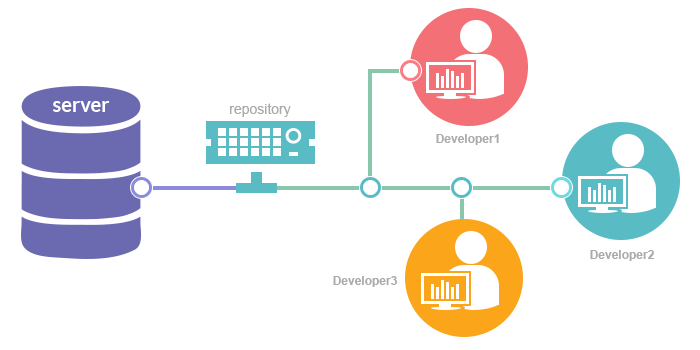
\includegraphics[width=7cm, keepaspectratio]{images/version_control.png}
				\end{center}
			\end{column}
		\end{columns}
	\end{frame}
	
	\begin{frame}{Lokális verziókezelők}
		\begin{columns}
			\begin{column}{0.5\textwidth}
				\only<1>{A legegyszerűbb verziókezelés, ha a fejlesztő kézzel átmásol egy mappába fájlokat. Ezek lehetnek idő bélyegzett mappák is, ha okos a fejlesztő. \par\smallskip
					Ez a megoldás nagyon egyszerű, viszont fogékony a hibákra, mert sok a manuális munka. Ezenkívül sok benne a redundáns adat is, mert a nem változtatott adatot is el kell tárolni. Ezért hozták létre a lokális verziókezelőket.}
				\only<2>{\begin{block}{Lokális verziókezelő}
						A lokális verziókezelők a teljes fájlok helyett csak a változtatásokat tárolják el egy külön erre kifejlesztett adatbázisban lokálisan, a számítógépen. Egy gyakori ilyen szoftver volt az RCS.
				\end{block}}
			\end{column}
			\begin{column}{0.5\textwidth}
				\begin{center}
					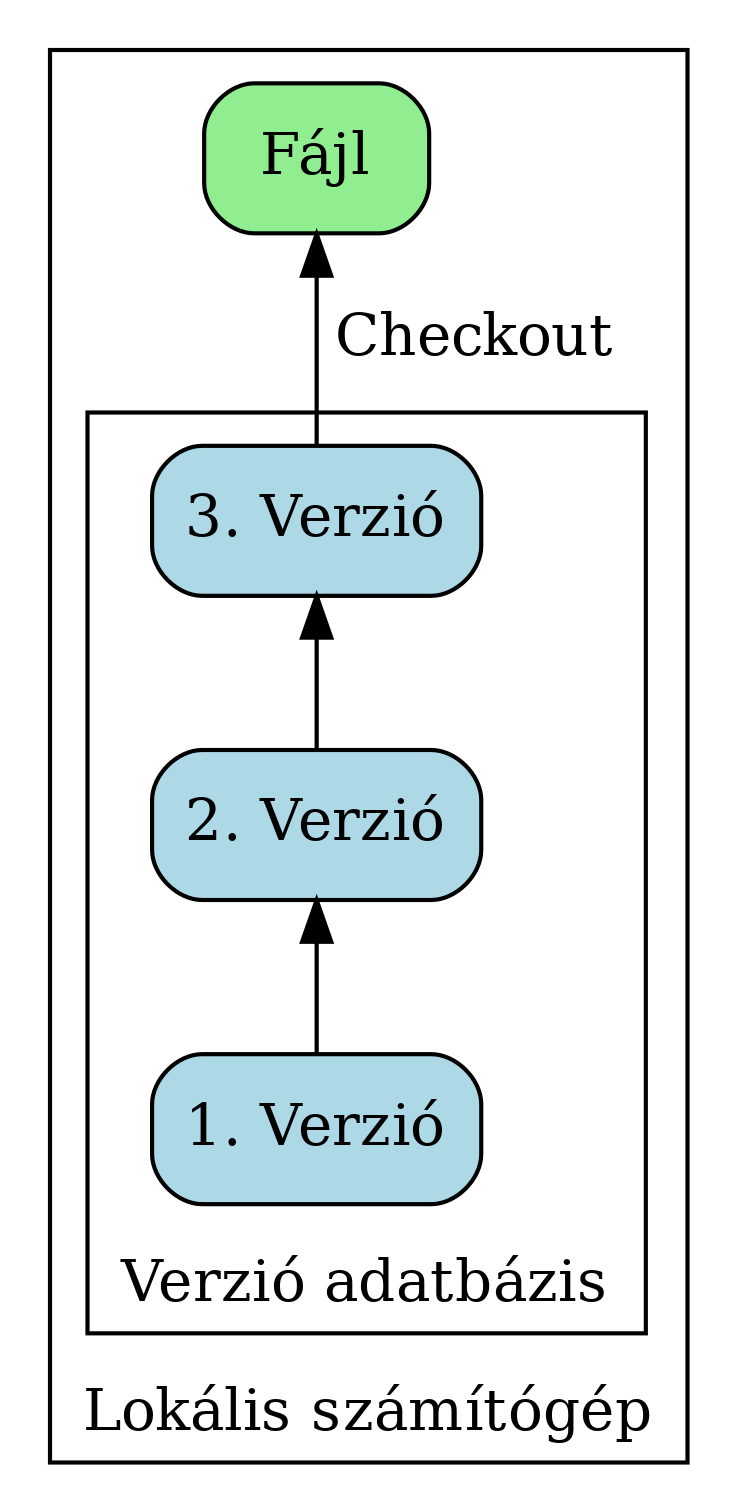
\includegraphics[width=7cm, height=7cm, keepaspectratio]{graphs/git_1.png}
				\end{center}
			\end{column}
		\end{columns}
	\end{frame}
	
	\begin{frame}{Centralizált verziókezelők}
		\begin{columns}
			\begin{column}{0.5\textwidth}
				\only<1>{A következő jelentős probléma, amivel az emberek találkoznak, az az, hogy együtt kell működniük fejlesztőkkel más rendszereken. Ennek a problémának a kezelésére Központosított Verziókezelő Rendszerek (CVCS-ek) lettek kifejlesztve.}
				\only<2>{\begin{block}{Centralizált verziókezelő}
						Ezek a rendszerek (például CVS, Subversion és Perforce) egyetlen szerverrel rendelkeznek, amely tartalmazza az összes verziózott fájlt, és számos klienst, akik a fájlokat ebből a központi helyről töltik be.
				\end{block}}
				\only<3>{Előnyei:
					\begin{itemize}
						\item Mindenki bizonyos mértékben tudja, hogy a projekt többi résztvevője mit csinál.
						\item Az adminisztrátorok részletes ellenőrzést gyakorolhatnak arról, hogy ki mit tehet meg, és sokkal könnyebb egy CVCS-t adminisztrálni, mint helyi adatbázisokkal foglalkozni minden kliens esetében.
				\end{itemize}}
				\only<4>{Hátrányai:
					\begin{itemize}
						\item Az egyetlen központi szerver hibapontot jelent, ahol akár egy órás leállás is lehetetlenné teszi a közös munkát és verziózási változtatások mentését.
						\item Adatvesztés veszélye, ha a központi adatbázis merevlemeze meghibásodik és nem rendelkezünk megfelelő biztonsági mentésekkel.
				\end{itemize}}
			\end{column}
			\begin{column}{0.5\textwidth}
				\begin{center}
					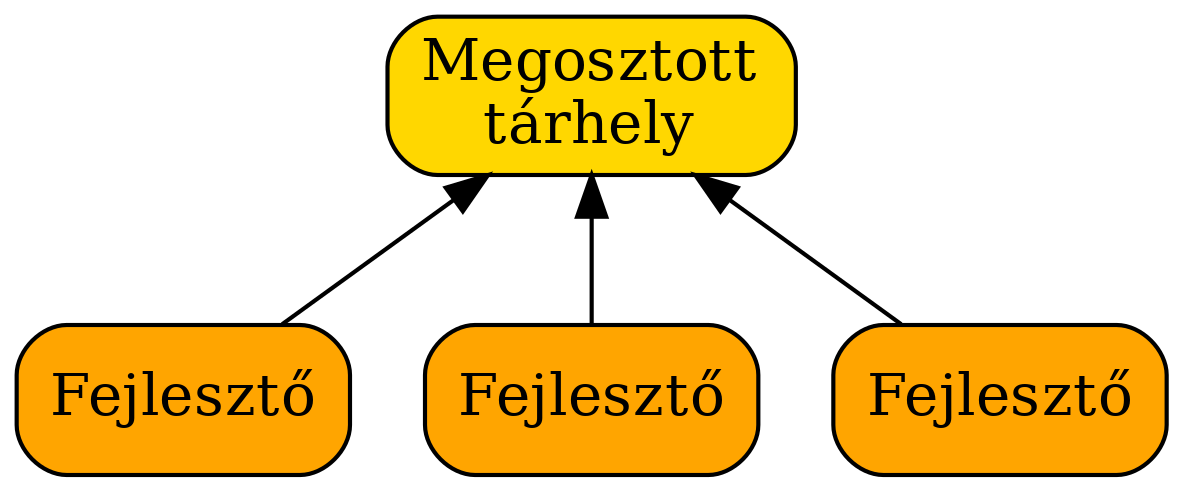
\includegraphics[width=7cm, keepaspectratio]{graphs/git_2.png}
				\end{center}
			\end{column}
		\end{columns}
	\end{frame}
	
	\begin{frame}{Elosztott verziókezelők}
		\begin{columns}
			\begin{column}{0.5\textwidth}
				\only<1>{Ebben a helyzetben lépnek képbe az elosztott verziókezelő rendszerek (DVCS-ek). Sok ilyen rendszer nagyon jól kezeli a több távoli tárolóval való együttműködést, így lehetőség van különböző emberekkel egyidejűleg egyazon projekt keretein belül együttműködni.}
				\only<2>{\begin{block}{Elosztott verziókezelő}
						A kliensek nem csak a fájlok legfrissebb pillanatképét töltik le, hanem teljes egészében tükrözik a tárhelyet, beleértve annak teljes előzményeit is. Ezért minden klón valójában egy teljes adatbiztonsági másolat.
				\end{block}}
			\end{column}
			\begin{column}{0.5\textwidth}
				\begin{center}
					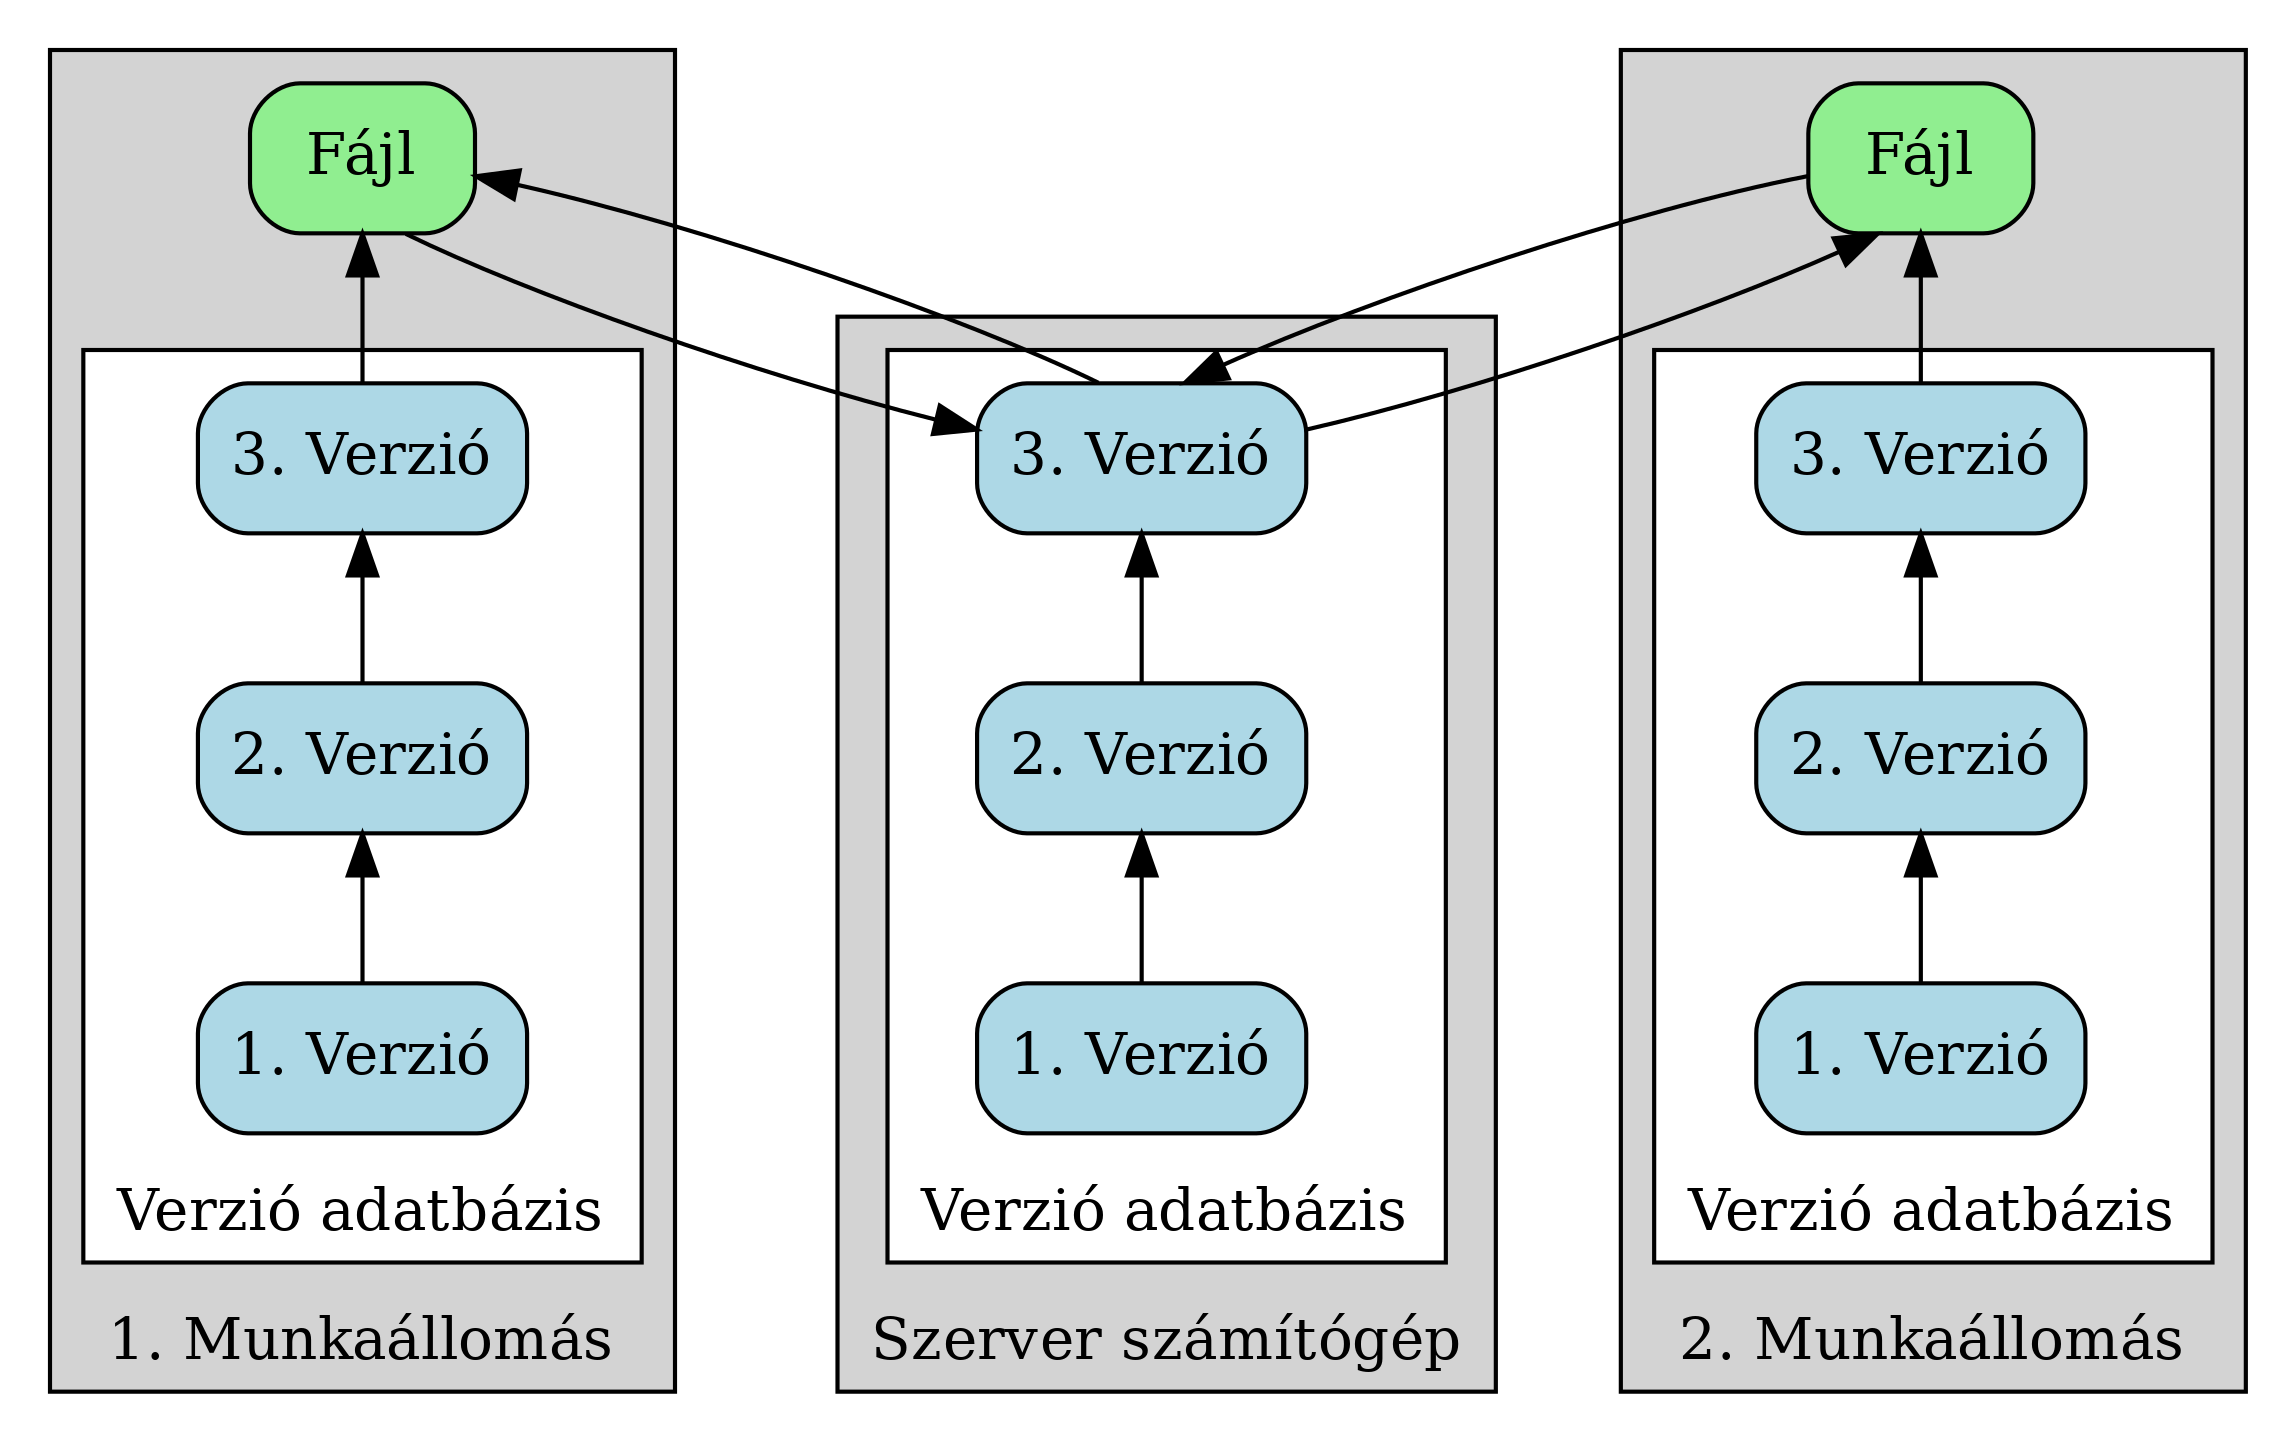
\includegraphics[height=7cm, width=7cm, keepaspectratio]{graphs/git_3.png}
				\end{center}
			\end{column}
		\end{columns}
	\end{frame}
	
	\section{Git alapok}
	
	\begin{frame}
		\tableofcontents[currentsection]
	\end{frame}
	
	\begin{frame}{A Git verziókezelő}
		\begin{columns}
			\begin{column}{0.5\textwidth}
				A Git úgy gondolkodik az adatokról, mint egy fájlrendszer pillanatképei.
				\\Segítségével minden alkalommal, amikor commit történik, (azaz elmentődik a projekt) készít egy képet arról, hogy az összes fájl hogyan néz ki abban a pillanatban, és eltárol egy hivatkozást erre a pillanatfelvételre. \par\smallskip
				A hatékonyság érdekében, ha a fájlok nem változtak, a Git nem tárolja újra a fájlt, csak egy hivatkozást az előző, azonos fájlra, amit már tárolt.
			\end{column}
			\begin{column}{0.5\textwidth}
				\begin{center}
					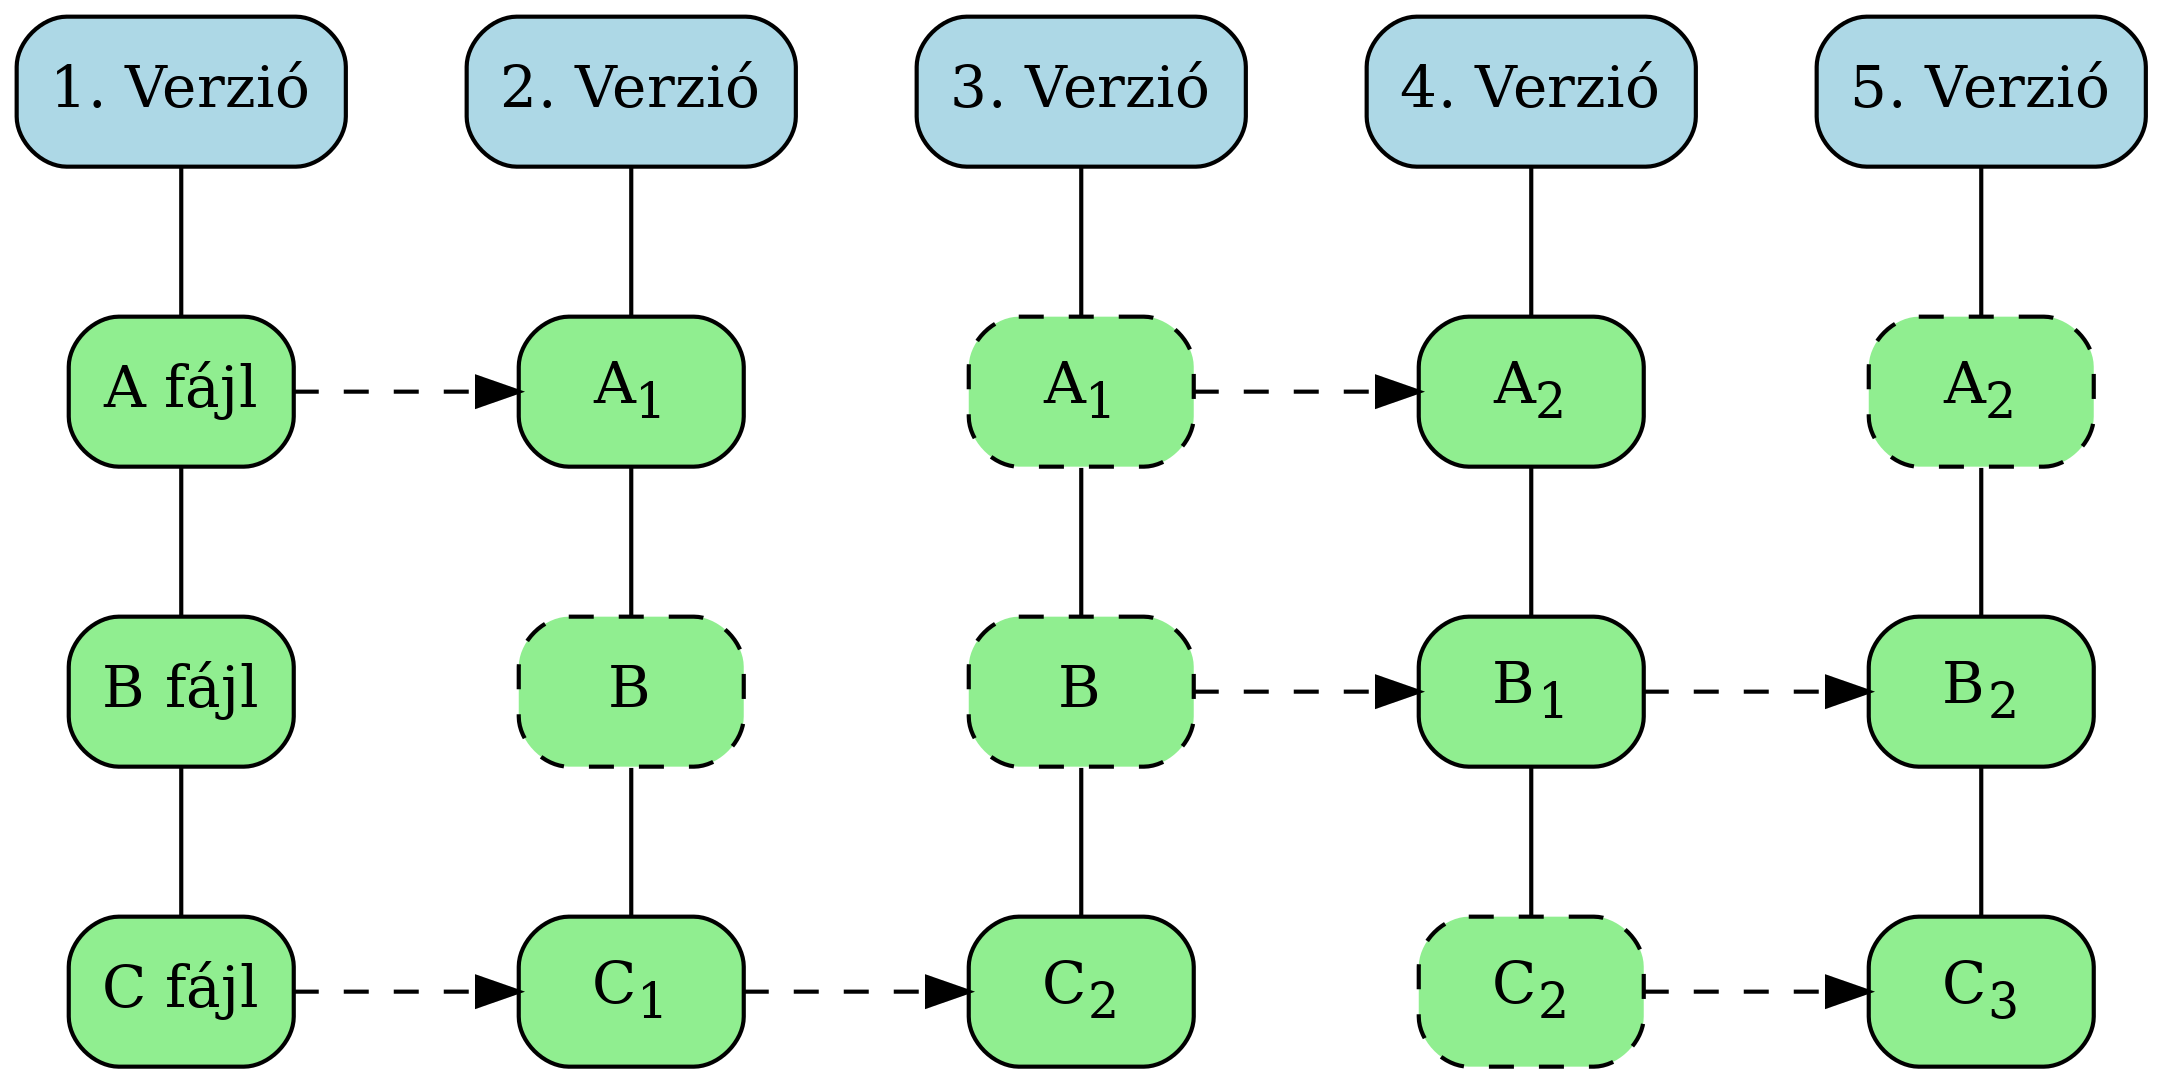
\includegraphics[width=7cm, keepaspectratio]{graphs/git_4.png}
				\end{center}
			\end{column}
		\end{columns}
	\end{frame}
	
	\begin{frame}{A három fájlállapot}
		\begin{columns}
			\begin{column}{0.5\textwidth}
				A Git rendszerében három fő állapota van a fájloknak: módosított (modified), megjelölt (staged) és tárolt (committed):
				\begin{itemize}
					\item A módosított azt jelenti, hogy a fájl meg lett változtatva, de még nem lett tárolva, sem tárolásra megjelölve
					\item A megjelölt állapot azt jelenti, hogy a módosított fájl az aktuális verziójában meg lett jelölve, hogy a következő commit pillanatképbe kerüljön
					\item A tárolt azt jelenti, hogy az adat biztonságosan tárolva van a helyi adatbázisban
				\end{itemize}
			\end{column}
			\begin{column}{0.6\textwidth}
				\begin{center}
					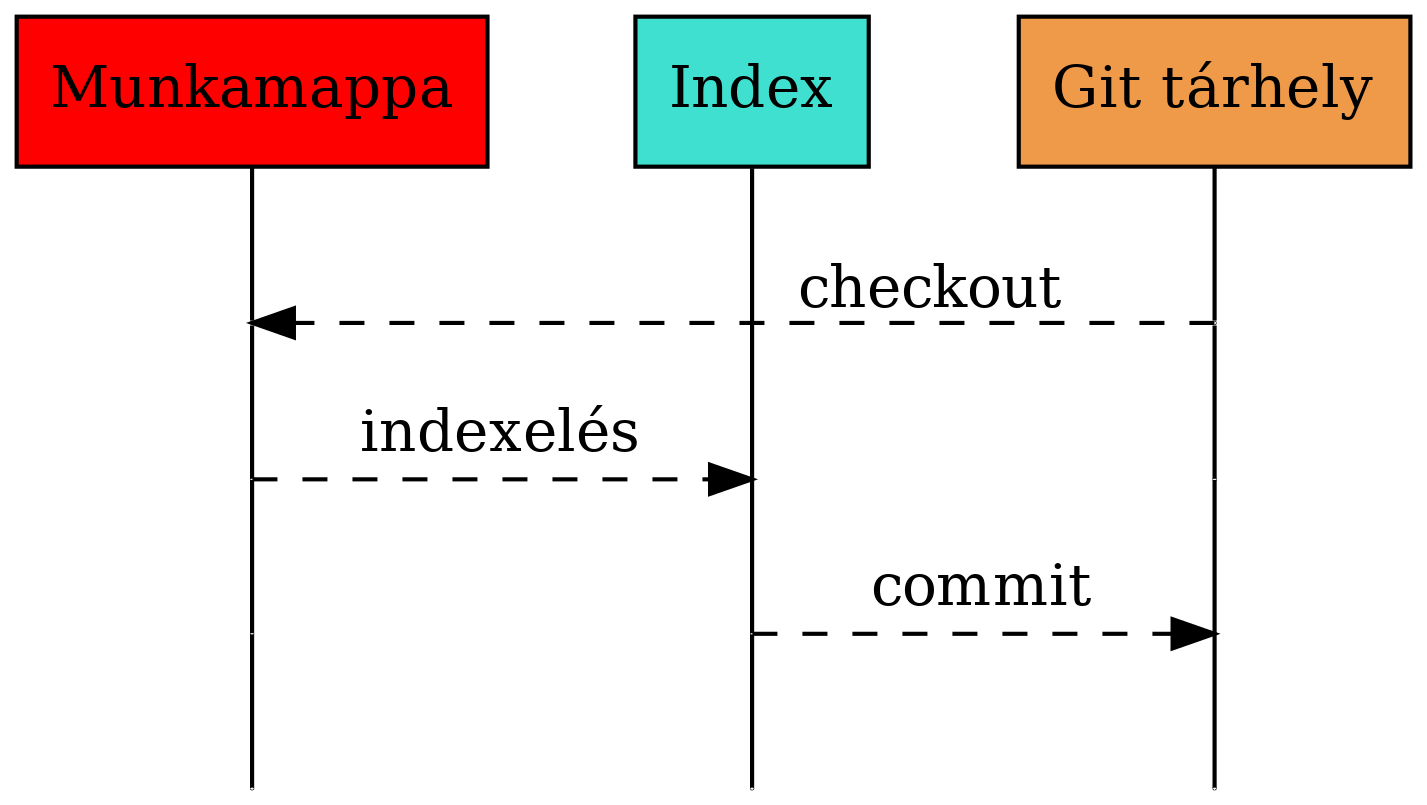
\includegraphics[width=8cm, height=8cm, keepaspectratio]{graphs/git_5.png}
				\end{center}
			\end{column}
		\end{columns}
	\end{frame}
	
	\begin{frame}{Státuszok változása}
		\begin{center}
			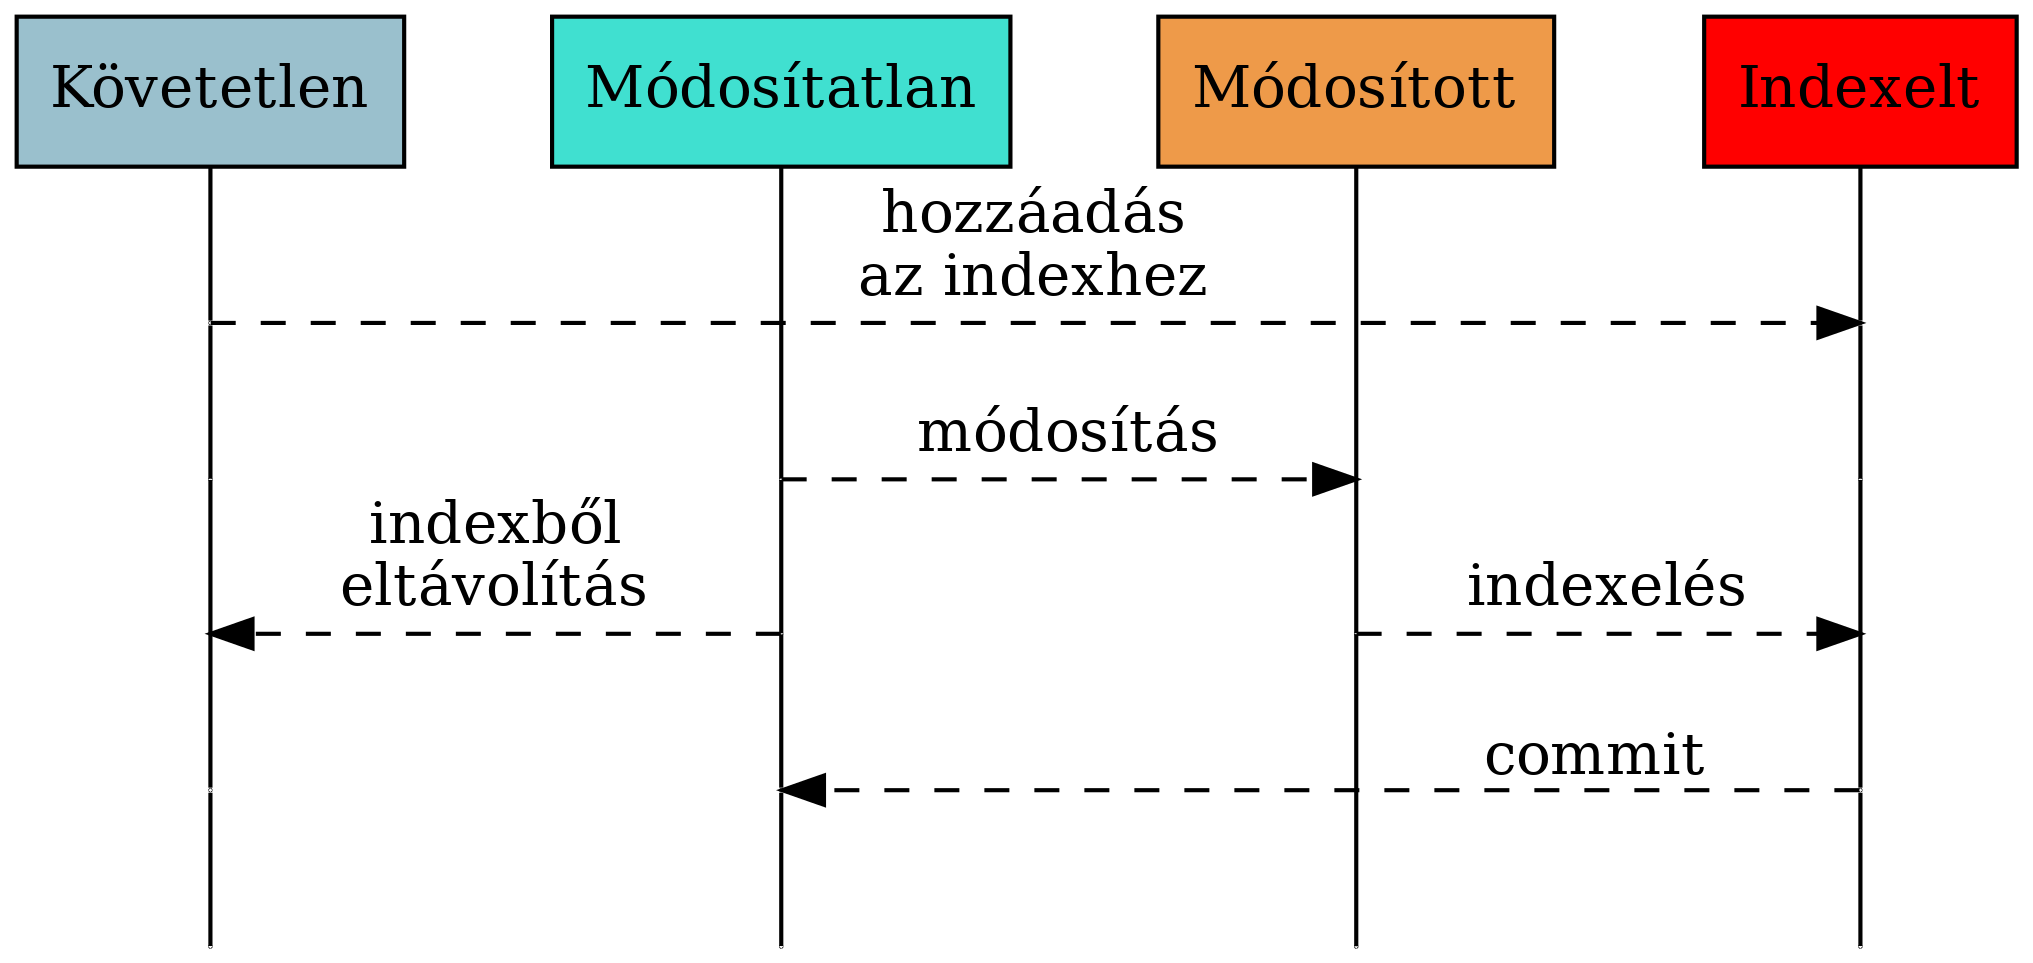
\includegraphics[width=14cm, keepaspectratio]{graphs/git_6.png}
		\end{center}
	\end{frame}
	
	\section{Git elágazások}
	
	\begin{frame}
		\tableofcontents[currentsection]
	\end{frame}
	
	\begin{frame}{Commitok tárolása}
		\begin{columns}
			\begin{column}{0.3\textwidth}
				\only<1>{Amikor a commit létrejön a \textbf{git commit} futtatásával, a Git  faobjektumként tárolja az adattárházban.\\
					Ezután a létrehoz egy \textbf{commit objektumot}, amely a metaadatokat és egy mutatót tartalmaz a gyökérprojekt fához, így azt újra létre tudja hozni szükség esetén.}
				\only<2>{\begin{center}
						\begin{block}{Commit}
							A \textbf{commit} a Git verziókezelő rendszerben egy olyan művelet, amely során a felhasználó rögzíti a változtatásokat a projektben, ezzel létrehozva egy új verziót az adattárházban. A commithoz commit üzenet társul.
						\end{block}
				\end{center}}
				\only<3>{A Git adattárház most öt objektumot tartalmaz:
					\begin{itemize}
						\item Három \textbf{blobot} (amelyek mindegyike egy-egy fájl tartalmát képviseli)
						\item Egy faobjektumot, amely felsorolja a könyvtár tartalmát és megadja, hogy mely fájlnevek tárolódnak mely blobokként
						\item Egy commitot a gyökérfa mutatójával és a metaadatokkal
				\end{itemize}}
			\end{column}
			\begin{column}{0.7\textwidth}
				\begin{center}
					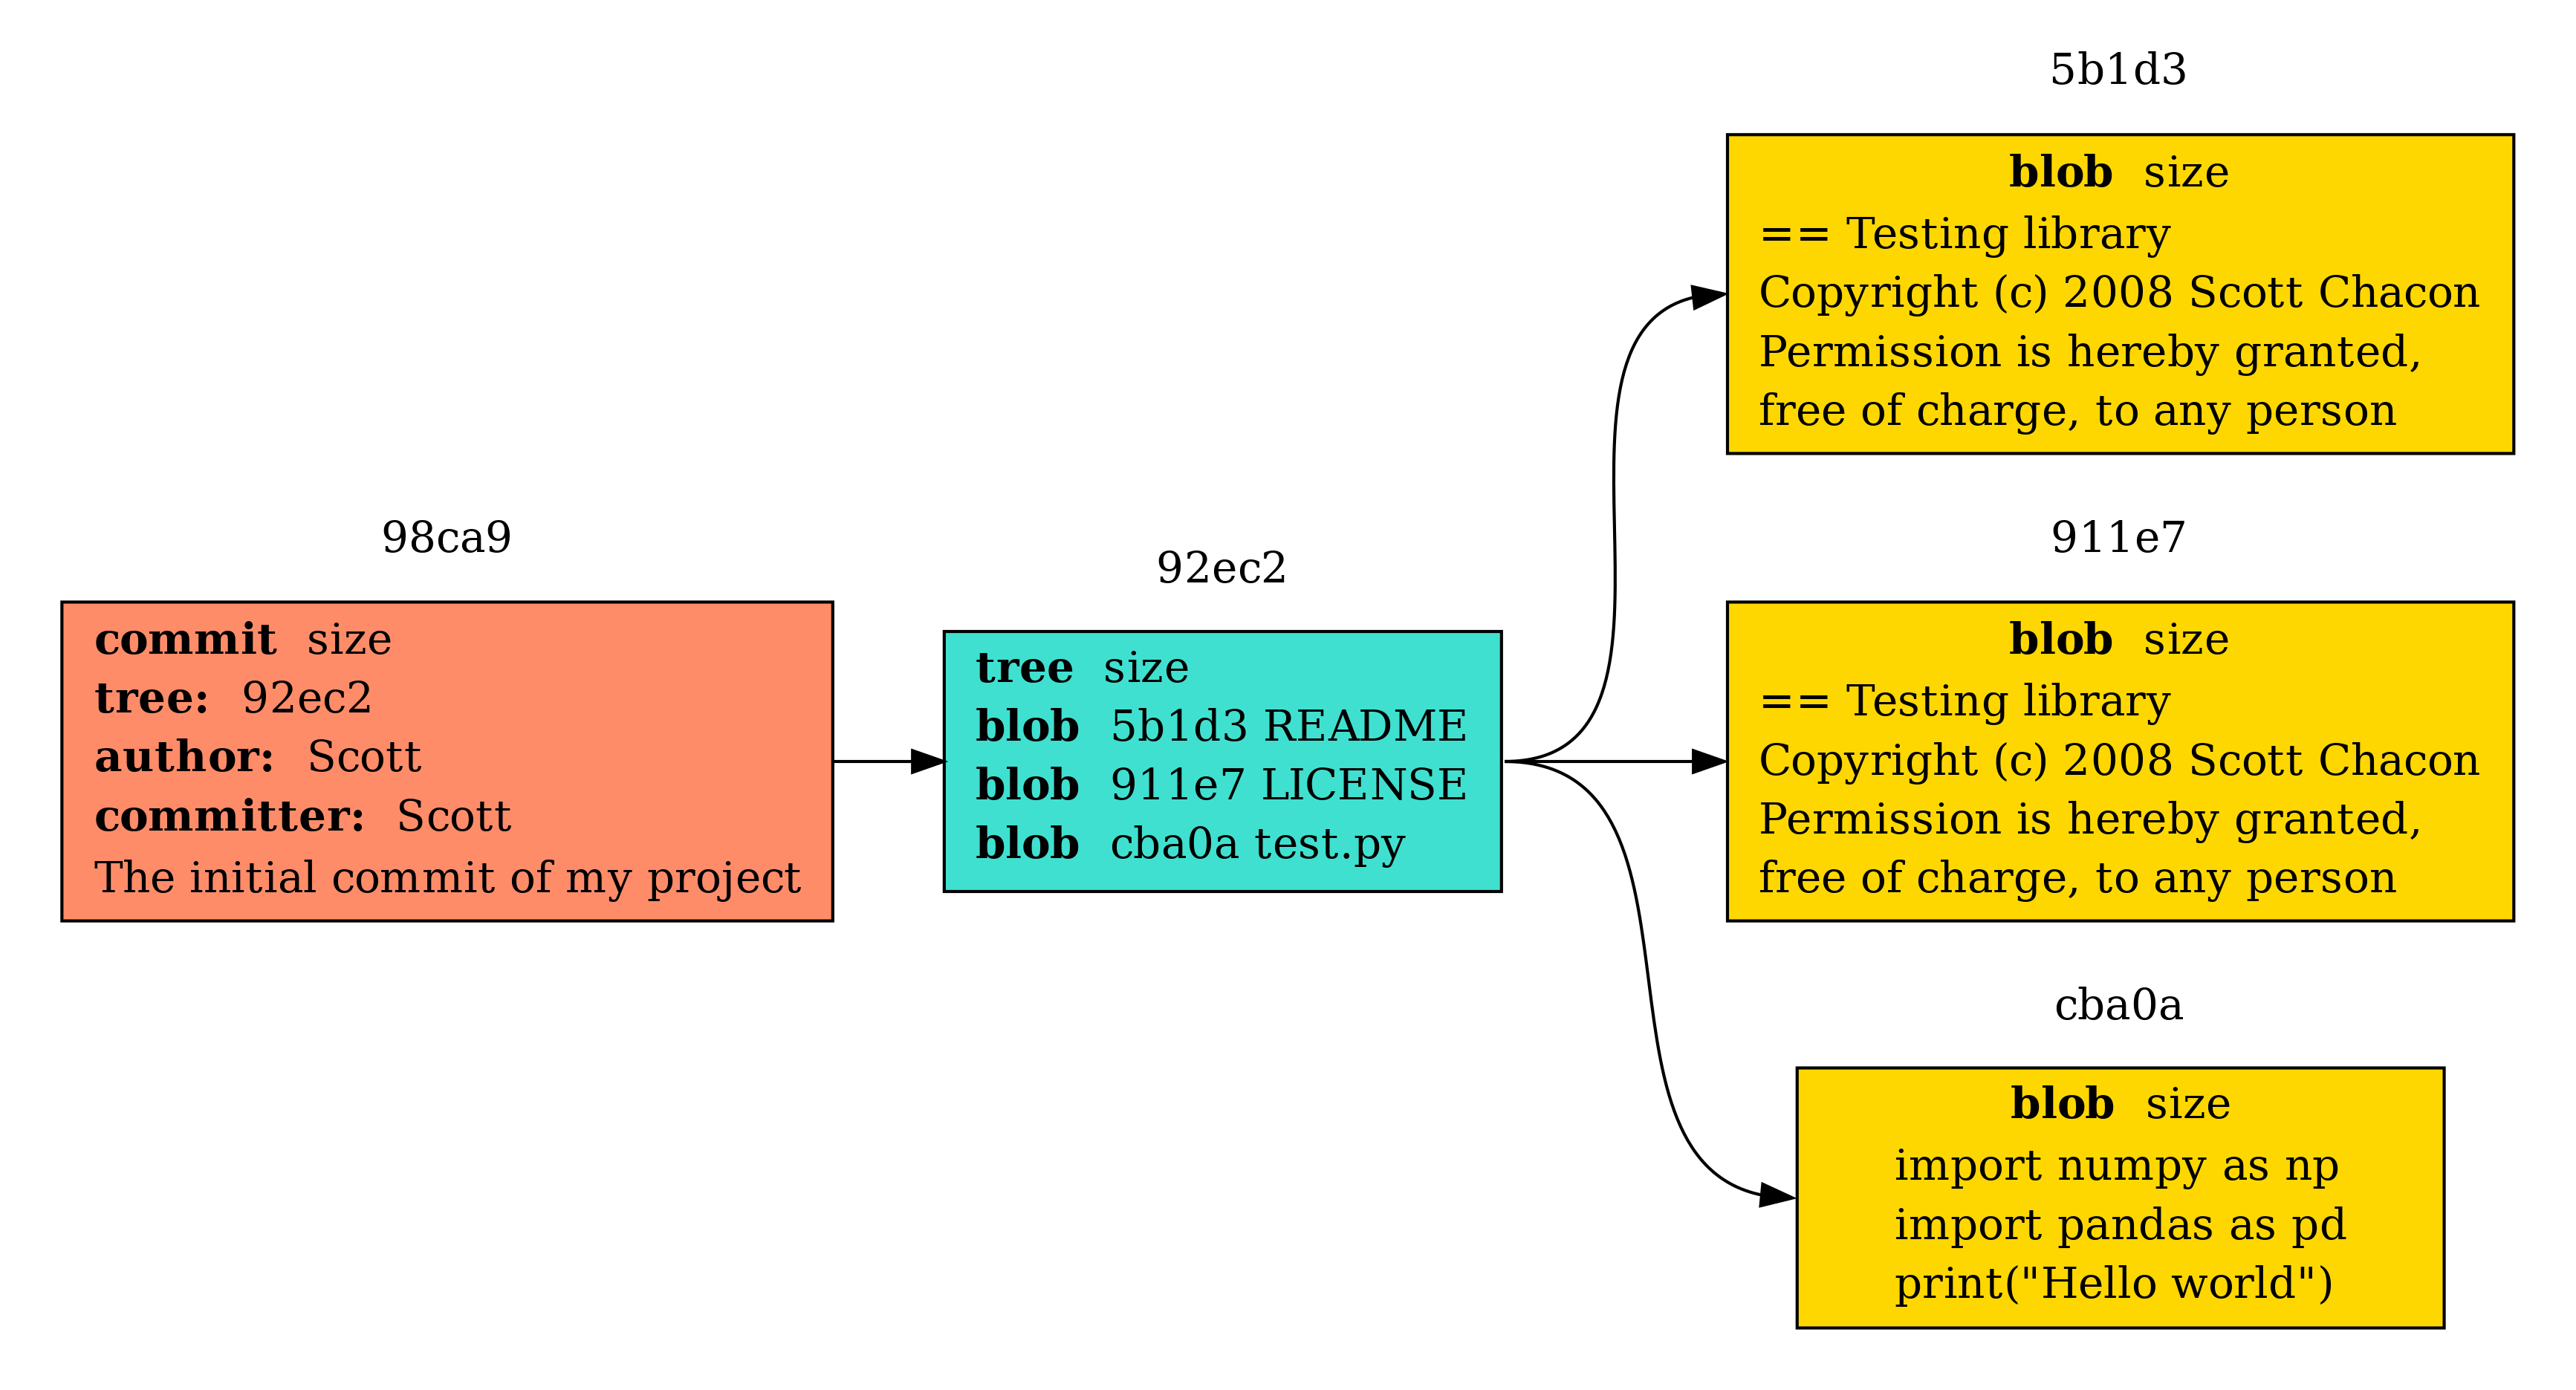
\includegraphics[width=10cm, height=10cm, keepaspectratio]{graphs/git_7.png}
				\end{center}
			\end{column}
		\end{columns}
	\end{frame}
	
	\begin{frame}{Több commit tárolása}
		\begin{columns}
			\begin{column}{.4\textwidth}
				Ha néhány változtatás után ismét egy commit következik, a következő commit egy mutatót tárol arra a commitra, amely közvetlenül megelőzte.\\
			\end{column}
			\begin{column}{.6\textwidth}
				\begin{center}
					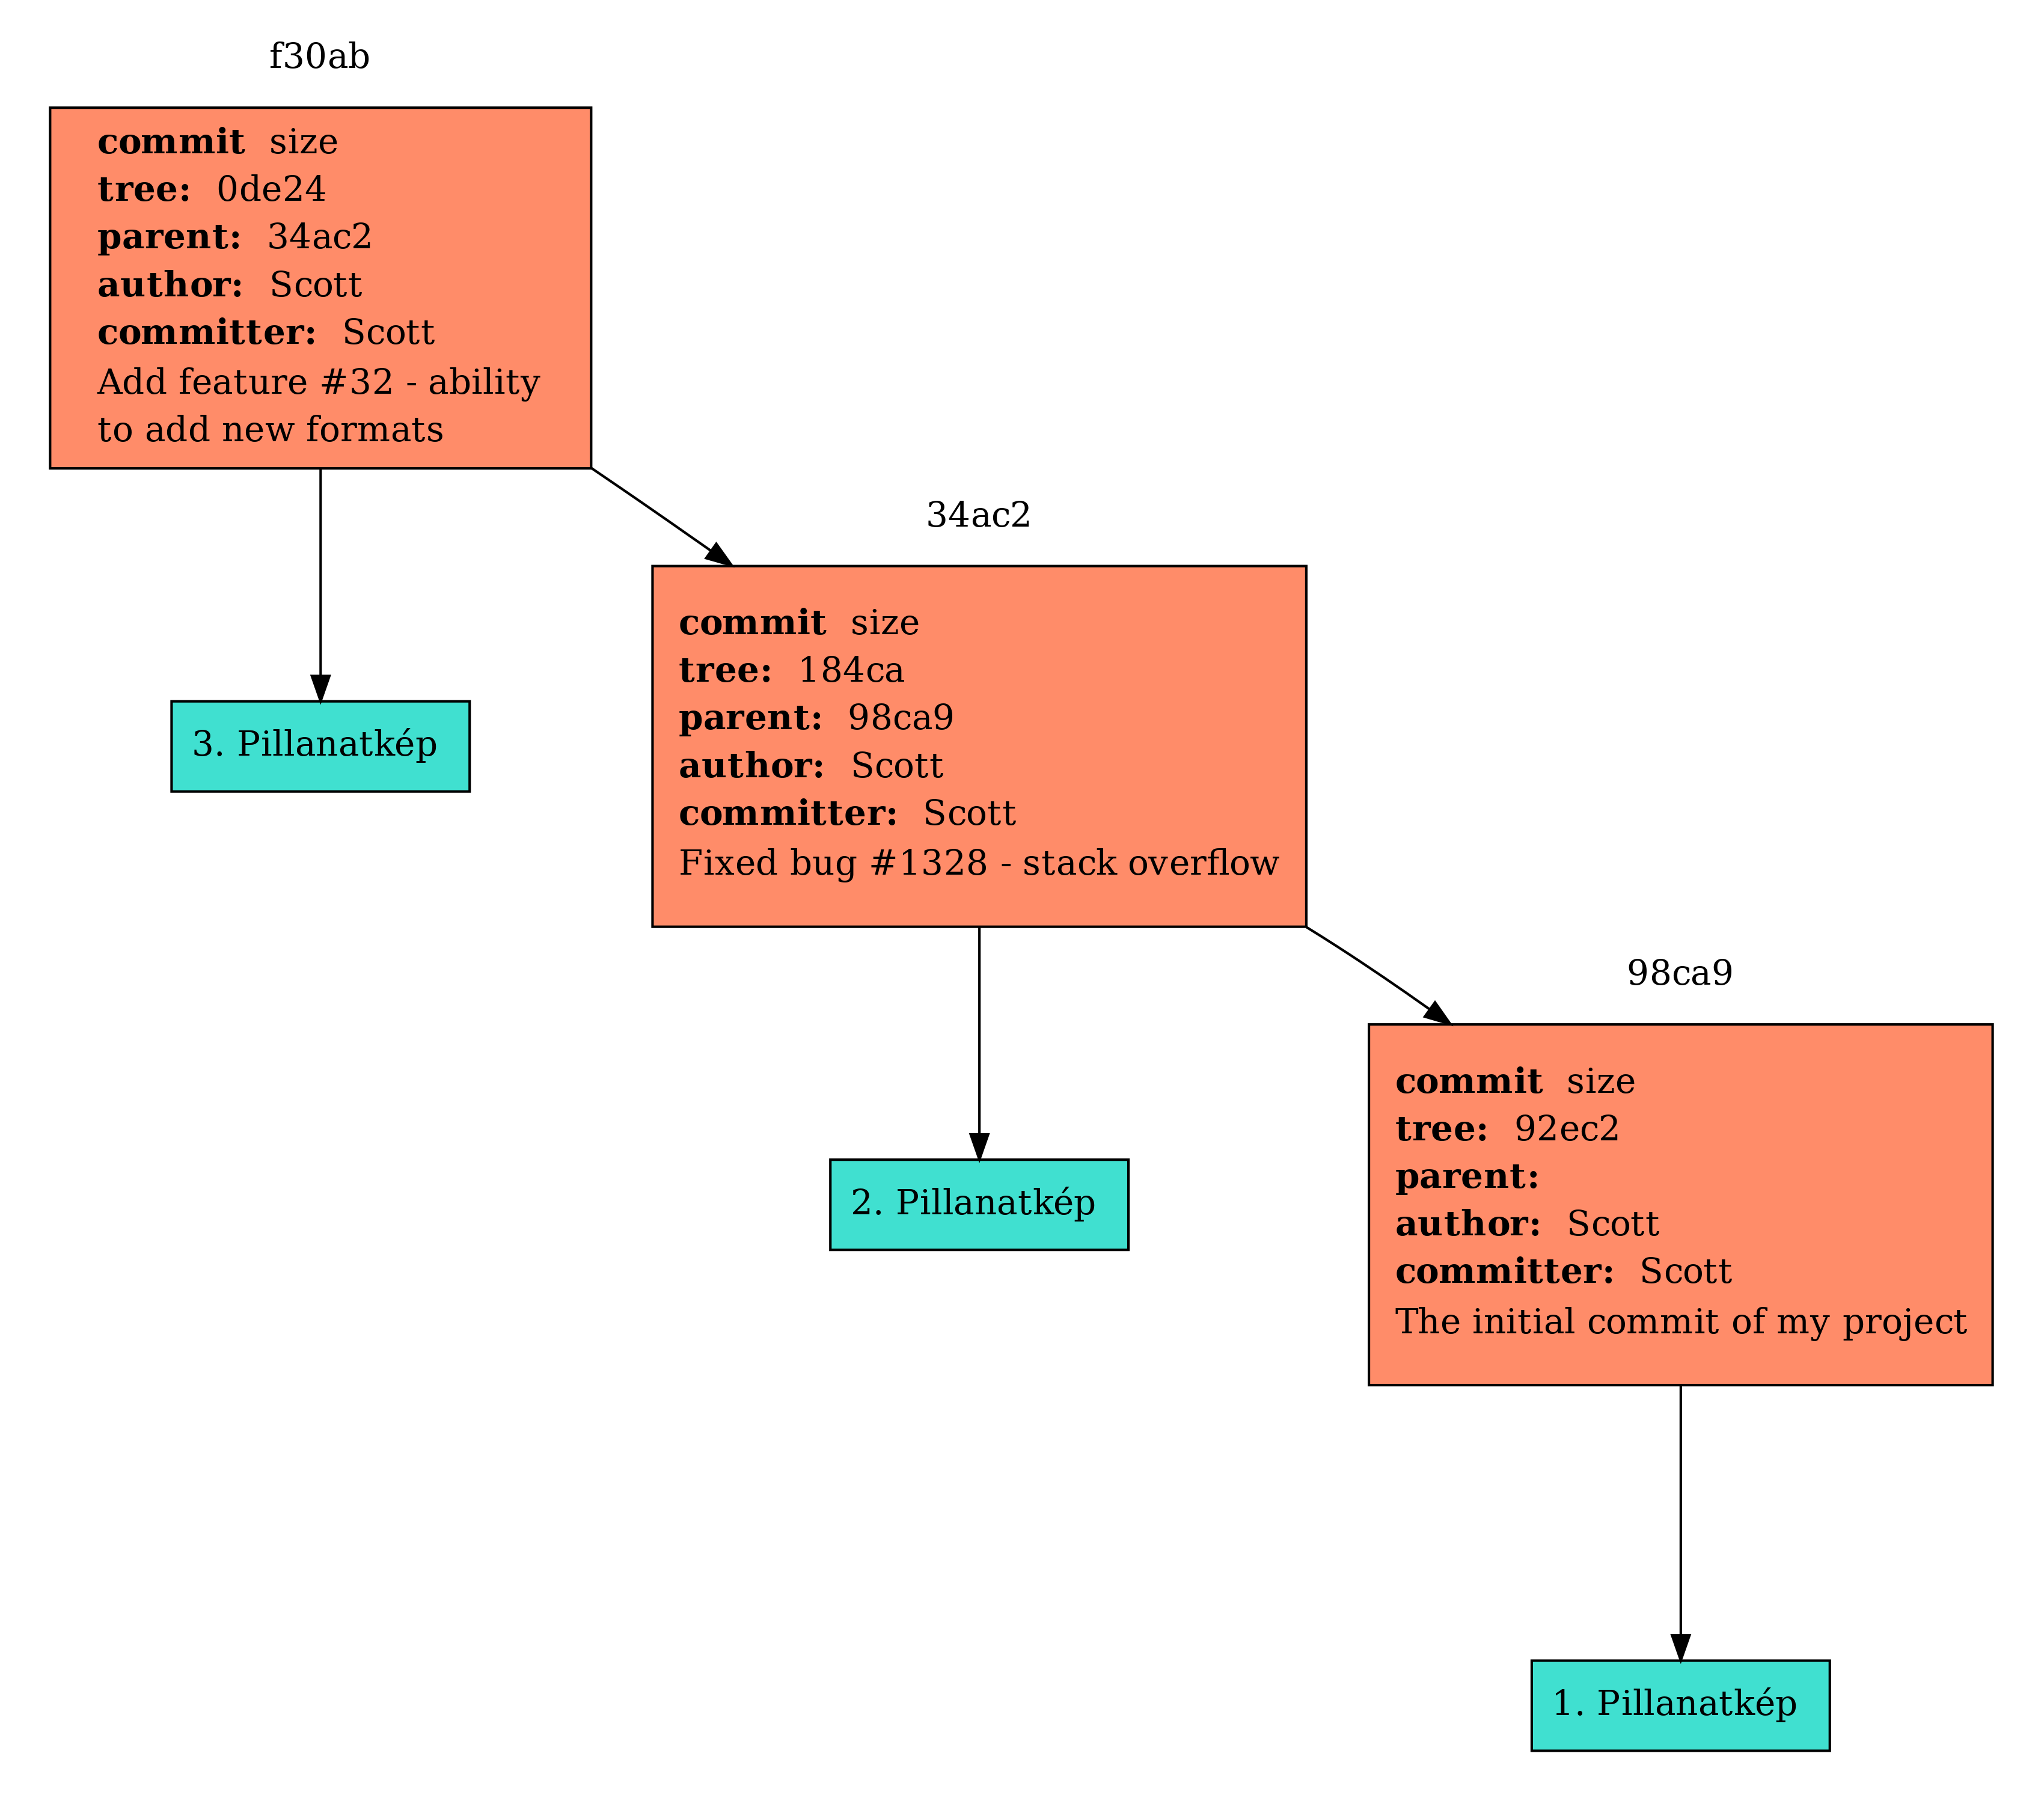
\includegraphics[height=7cm, keepaspectratio]{graphs/git_8.png}
				\end{center}
			\end{column}
		\end{columns}
	\end{frame}
	
	\begin{frame}{Egy Git ág és az előzményei}
		\begin{columns}
			\begin{column}{0.4\textwidth}
				\only<1>{\begin{block}{Fejlesztési ág}
						A Gitben egy \textbf{fejlesztési ág} egy egyszerű mozgatható mutató, amely valamely commitra mutat.\\
						\vspace{0.2cm}
						A példában fejlesztési ágak a \texttt{v1.0} és \texttt{master}.
				\end{block}}
				\only<2>{Az alapértelmezett ágnév a Gitben a \textbf{master}. Ahogy a commitok készülnek, a projekt kap egy master ágat, amely az utolsó, a felhasználó által készített commitra mutat. Minden egyes commitkor a master ág mutatója automatikusan előre mozog.}
				\only<3>{\begin{block}{HEAD}
						A Git egy speciális mutatót tart nyilván, ami a \textbf{HEAD} néven ismert: ez egy mutató a jelenlegi helyi ágra. \\
						Új fejlesztési ág létrehozásakor a HEAD nem az új ágra mutat, ezt kézzel kell megváltoztatni. Ez a \textbf{checkout}.
				\end{block}}
			\end{column}
			\begin{column}{0.6\textwidth}
				\begin{center}
					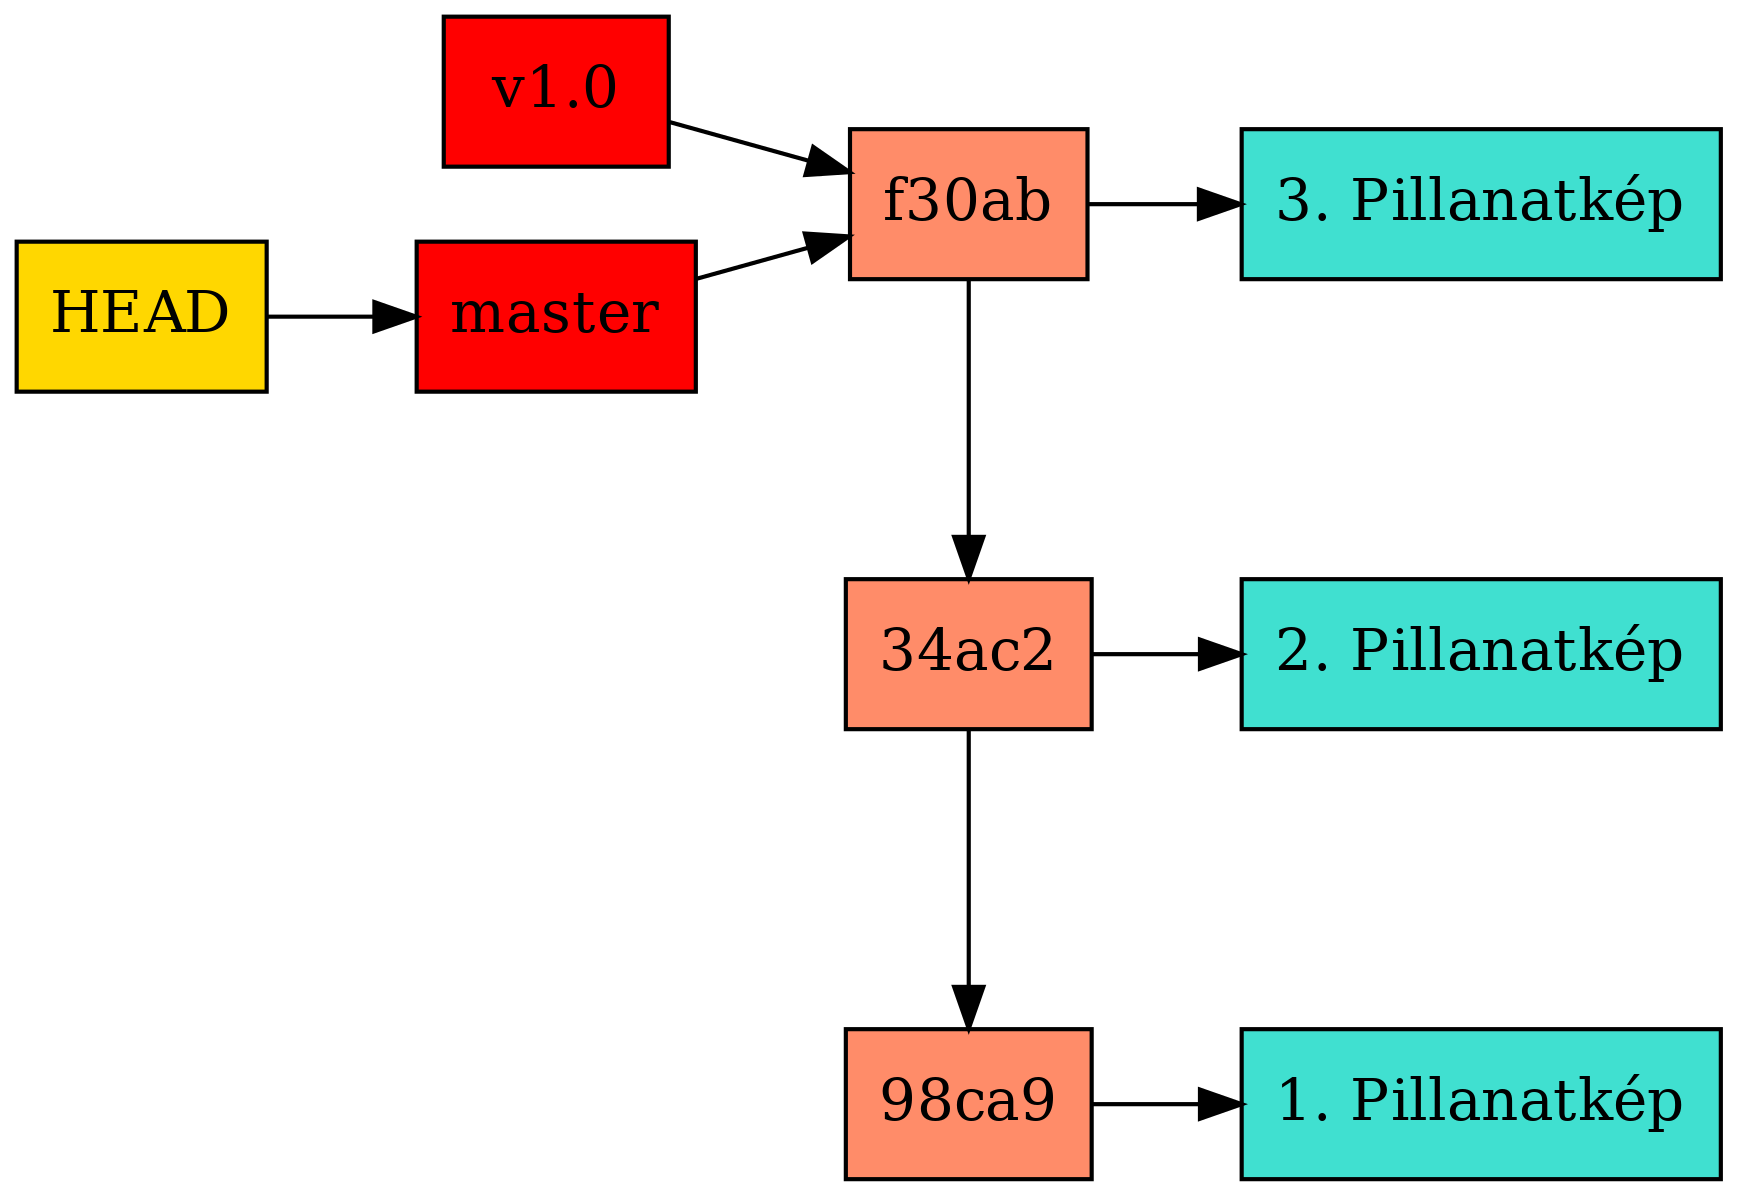
\includegraphics[width=9cm, height=9cm, keepaspectratio]{graphs/git_9.png}
				\end{center}
			\end{column}
		\end{columns}
	\end{frame}
	
	\begin{frame}{Checkout}
		\only<1>{
			Amikor új ágat hozunk létre, egy új mutató jön létre a verziókezelőben. Ebben az esetben a HEAD még az eredeti ágra mutat.
			\begin{center}
				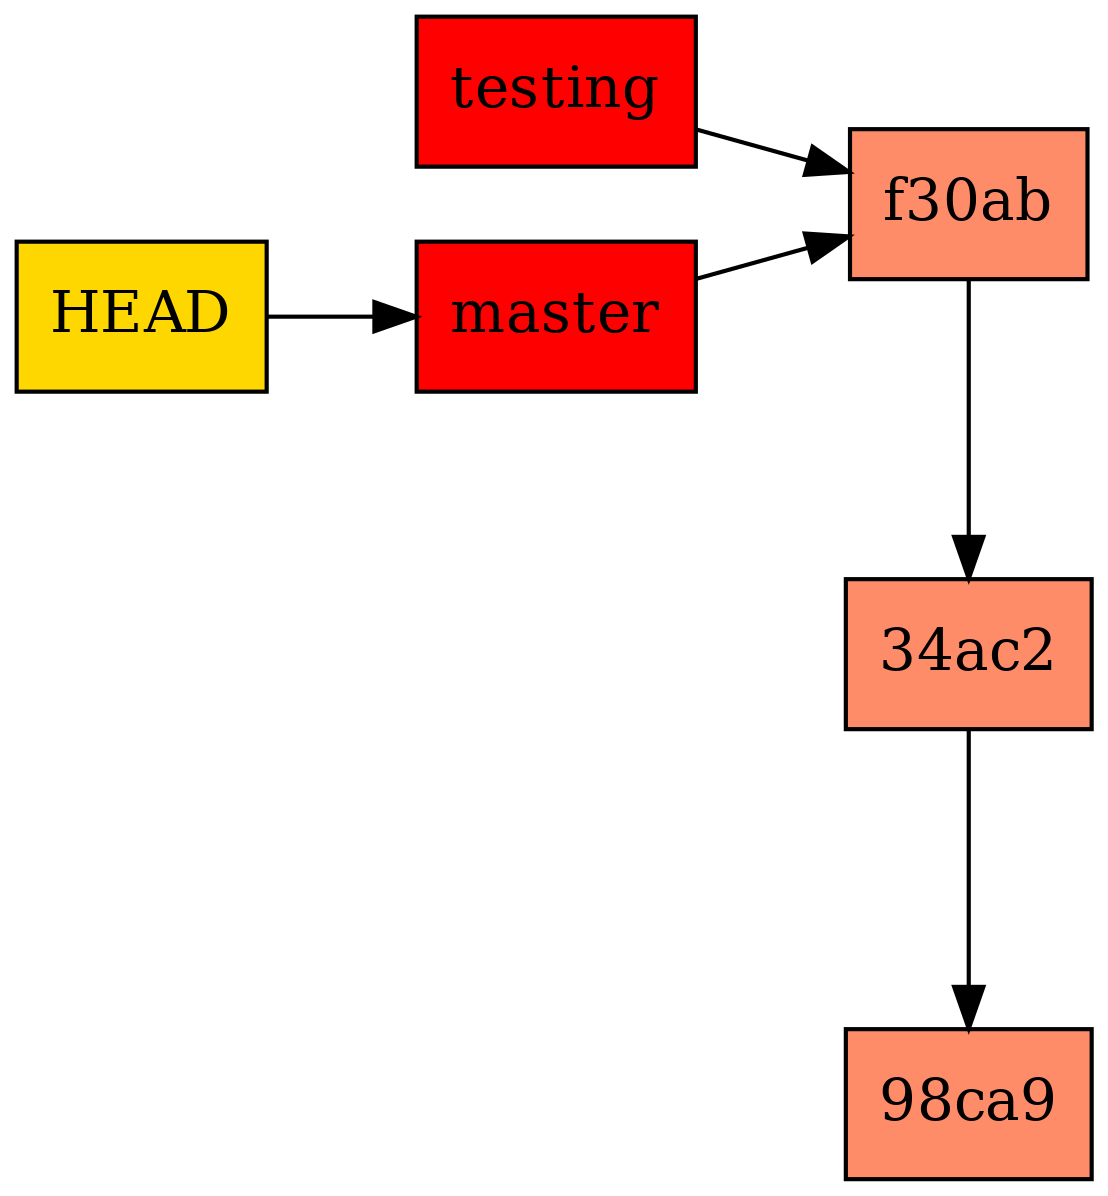
\includegraphics[height=6cm, keepaspectratio]{graphs/git_10.png}
		\end{center}}
		\only<2>{
			A checkout művelete átírja a HEAD mutató pozícióját a megjelölt fejlesztési ágra.
			\begin{center}
				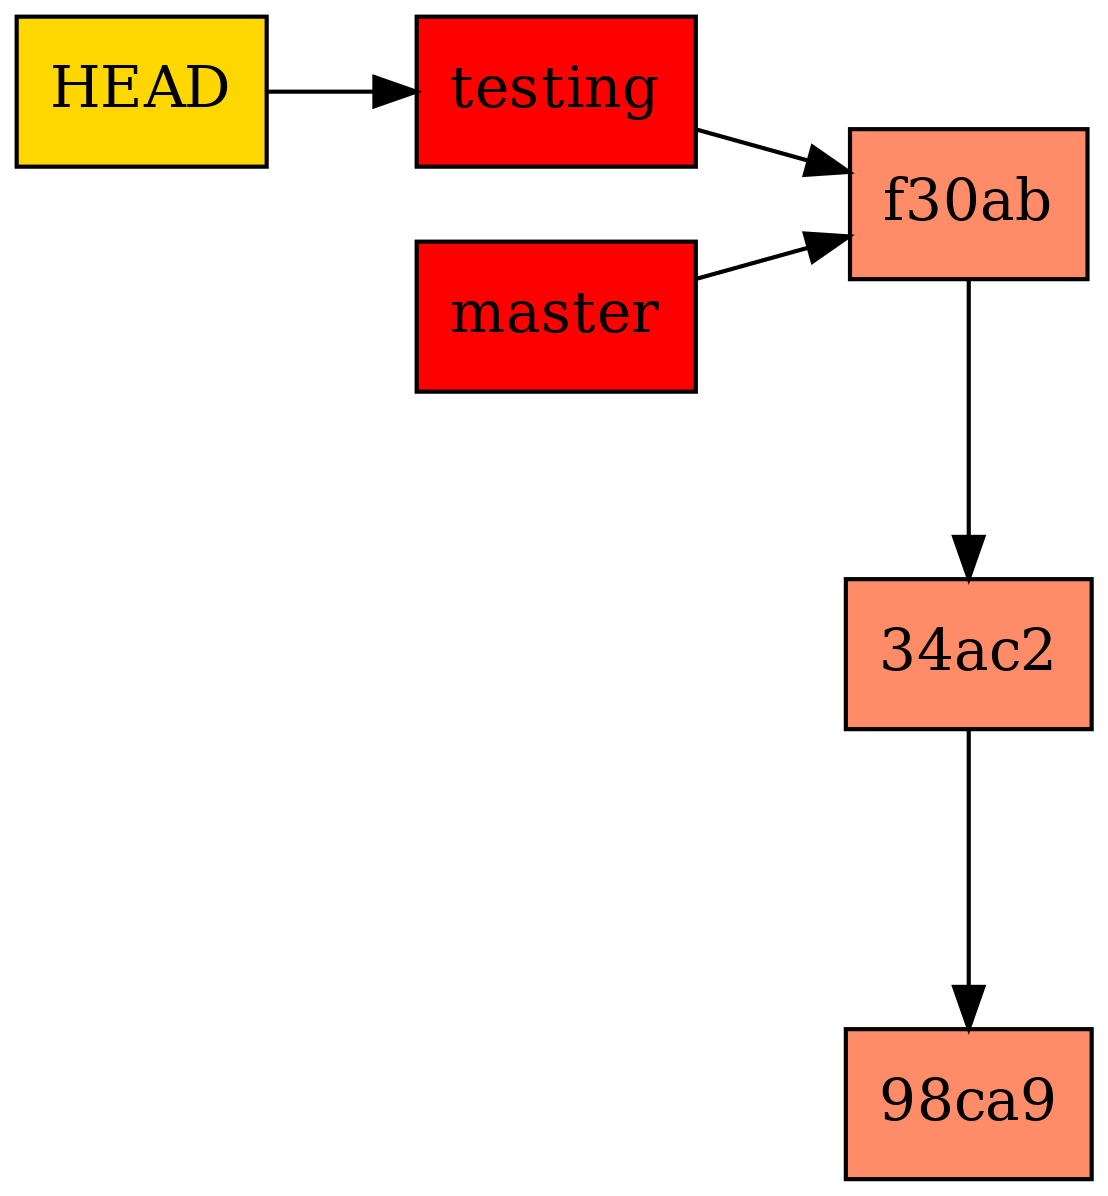
\includegraphics[height=6cm, keepaspectratio]{graphs/git_11.png}
		\end{center}}
	\end{frame}
	
	\begin{frame}{Commit az új ágra}
		Ha a jelenleg aktív (checkout által megjelölt) fejlesztési ágra történik egy commit, az ág lehagyja a main-t 1 commit-tal.
		\begin{center}
			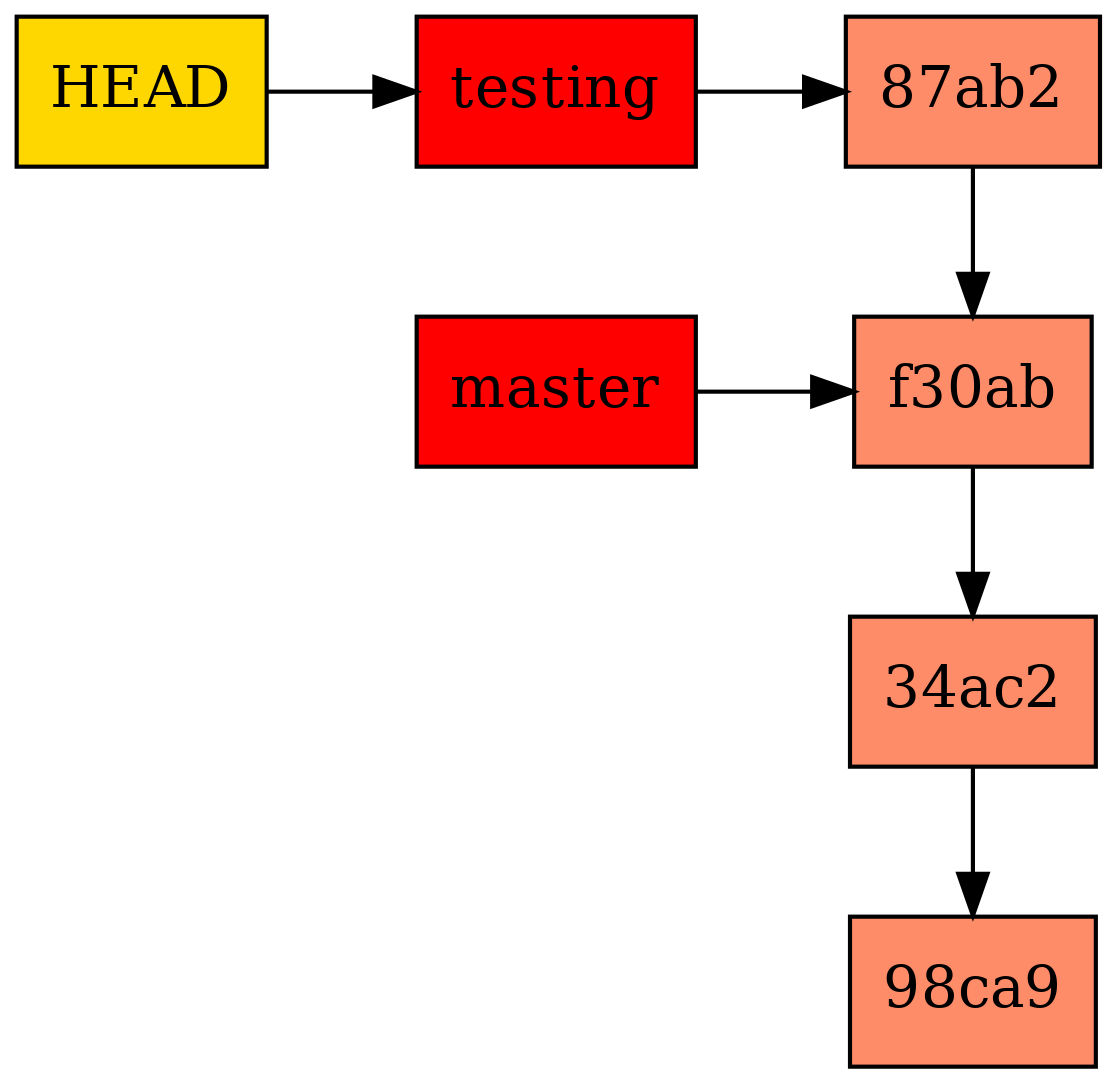
\includegraphics[height=6cm, width=14cm, keepaspectratio]{graphs/git_12.png}
		\end{center}
	\end{frame}
	
	\begin{frame}{Másik ág aktiválása}
		A fejlesztési ágak között szabadon lehet váltani. Ha a checkout művelettel aktiválódik a master ág, a HEAD mutató onnantól kezdve rá mutat. Ebben az esetben a mappában lévő fájlok is megváltoznak a master-ben elmentett állapotukra.
		\begin{center}
			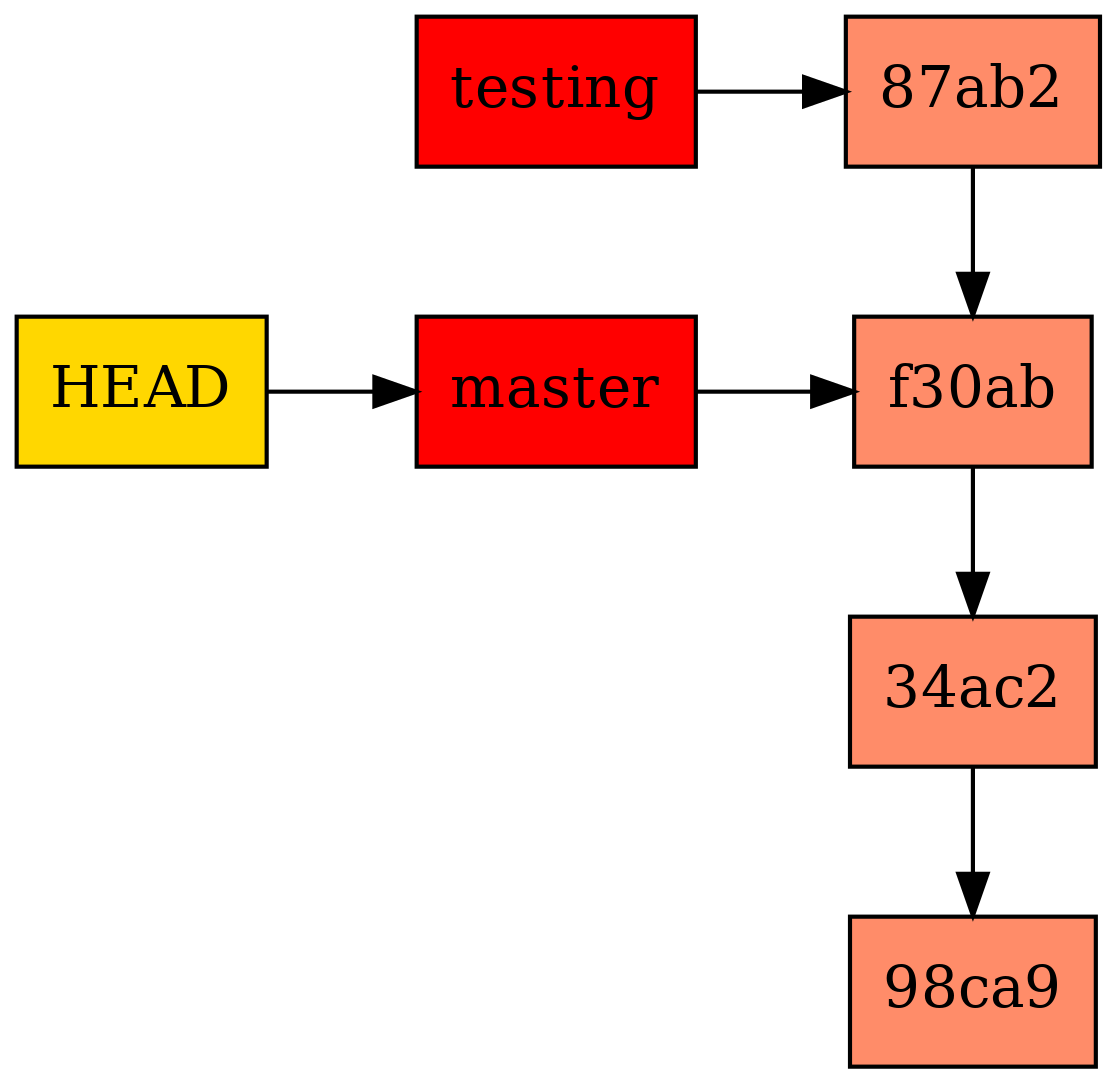
\includegraphics[height=5cm, width=14cm, keepaspectratio]{graphs/git_13.png}
		\end{center}
	\end{frame}
	
	\begin{frame}{Commit a master ágra}
		Ha ebben az állapotban a master ágra érkezik egy commit, egy új főág nyílik a projekten belül, és a két ág (testing, master) külön válnak.
		\begin{center}
			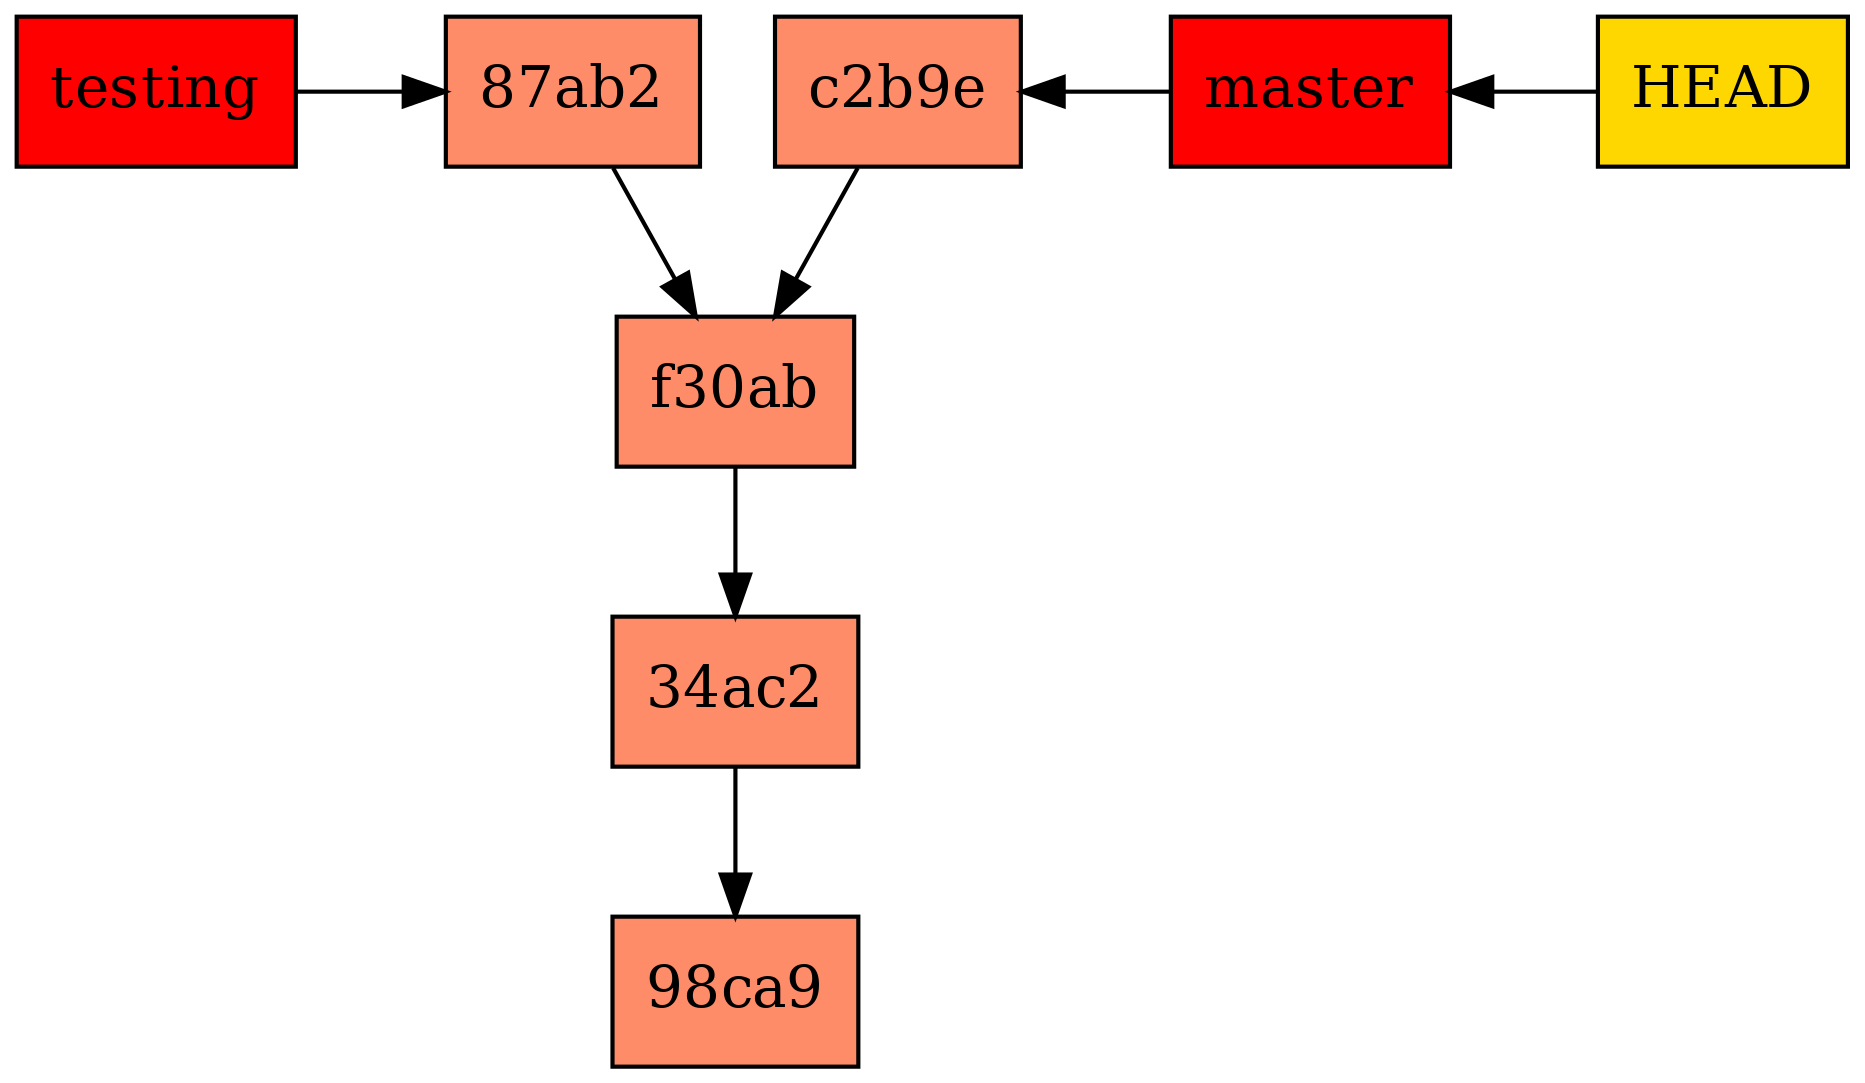
\includegraphics[height=6cm, width=14cm, keepaspectratio]{graphs/git_14.png}
		\end{center}
	\end{frame}
	
	\section{Több ág kezelése}
	
	\begin{frame}
		\tableofcontents[currentsection]
	\end{frame}
	
	\begin{frame}{Hosszan futó fejlesztési ágak}
		\only<1>{
			Sok Git fejlesztő alkalmaz egy olyan munkafolyamatot, amely azt a megközelítést követi, hogy csak teljesen stabil kódot tartanak a \texttt{master} ágon.\\
			\vspace{0.2cm}
			Van egy másik párhuzamos águk, amit \texttt{develop} vagy \texttt{next} néven neveznek, amelyen dolgoznak vagy a stabilitást tesztelik. Ezt használják a témakör ágak beolvasztására, amikor készen állnak, hogy megbizonyosodjanak arról, hogy minden teszt átment és nem vezetnek be hibákat.\\
			\vspace{0,2cm}
			Valójában arról beszélünk, hogy a mutatók feljebb mozognak a készített commitok sorában. A stabil ágak lejjebb vannak a commit történetben, míg a legújabb fejlesztések ágai feljebb találhatók.
			\begin{center}
				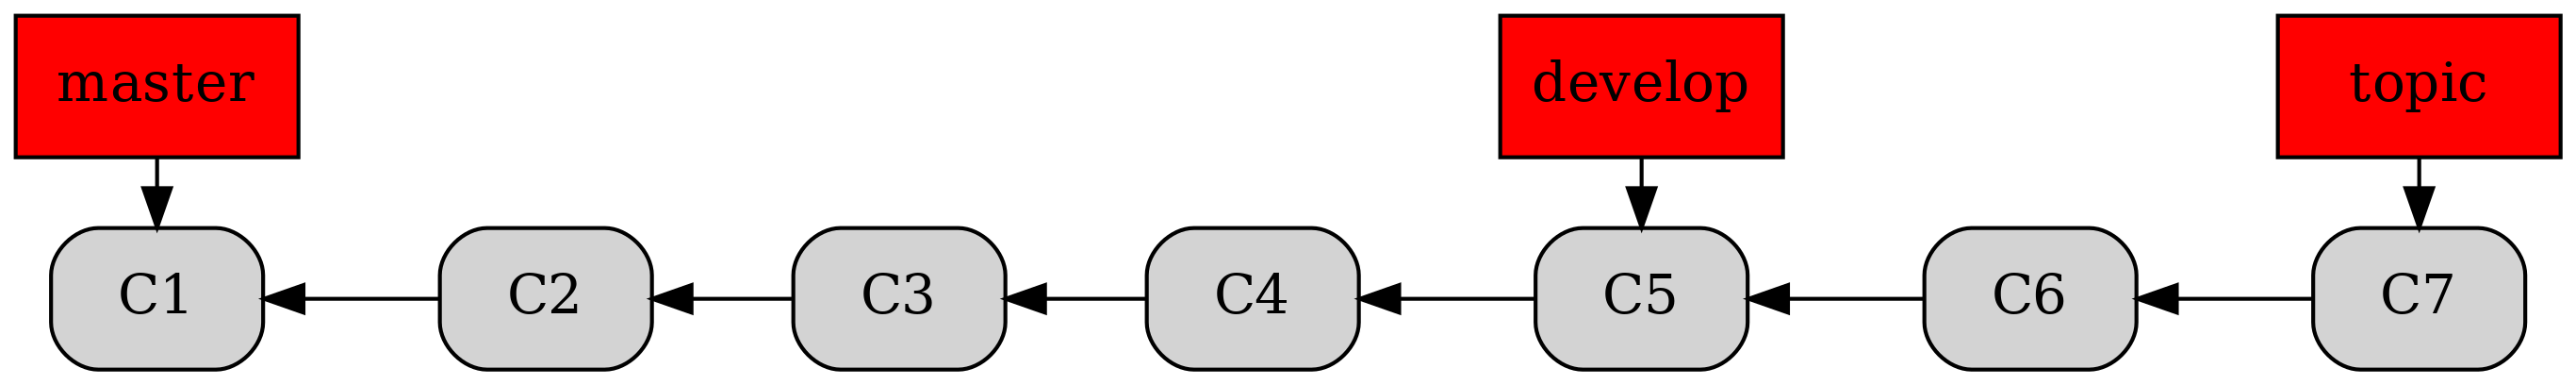
\includegraphics[width=14cm, height=7cm, keepaspectratio]{graphs/git_21.png}
		\end{center}}
		\only<2>{
			Ezzel ekvivalens definíció, ha a fejlesztési ágak külön-külön silókban vannak ábrázolva. Ezt lehetséges tovább végezni több szinten keresztül, de az általános elv a fejlesztési ágak létrehozására, hogy különböző stabilitási szintekkel rendelkeznek. Amikor egy ág elér egy stabilabb állapotot, akkor beolvad a felette lévőbe.
			\begin{center}
				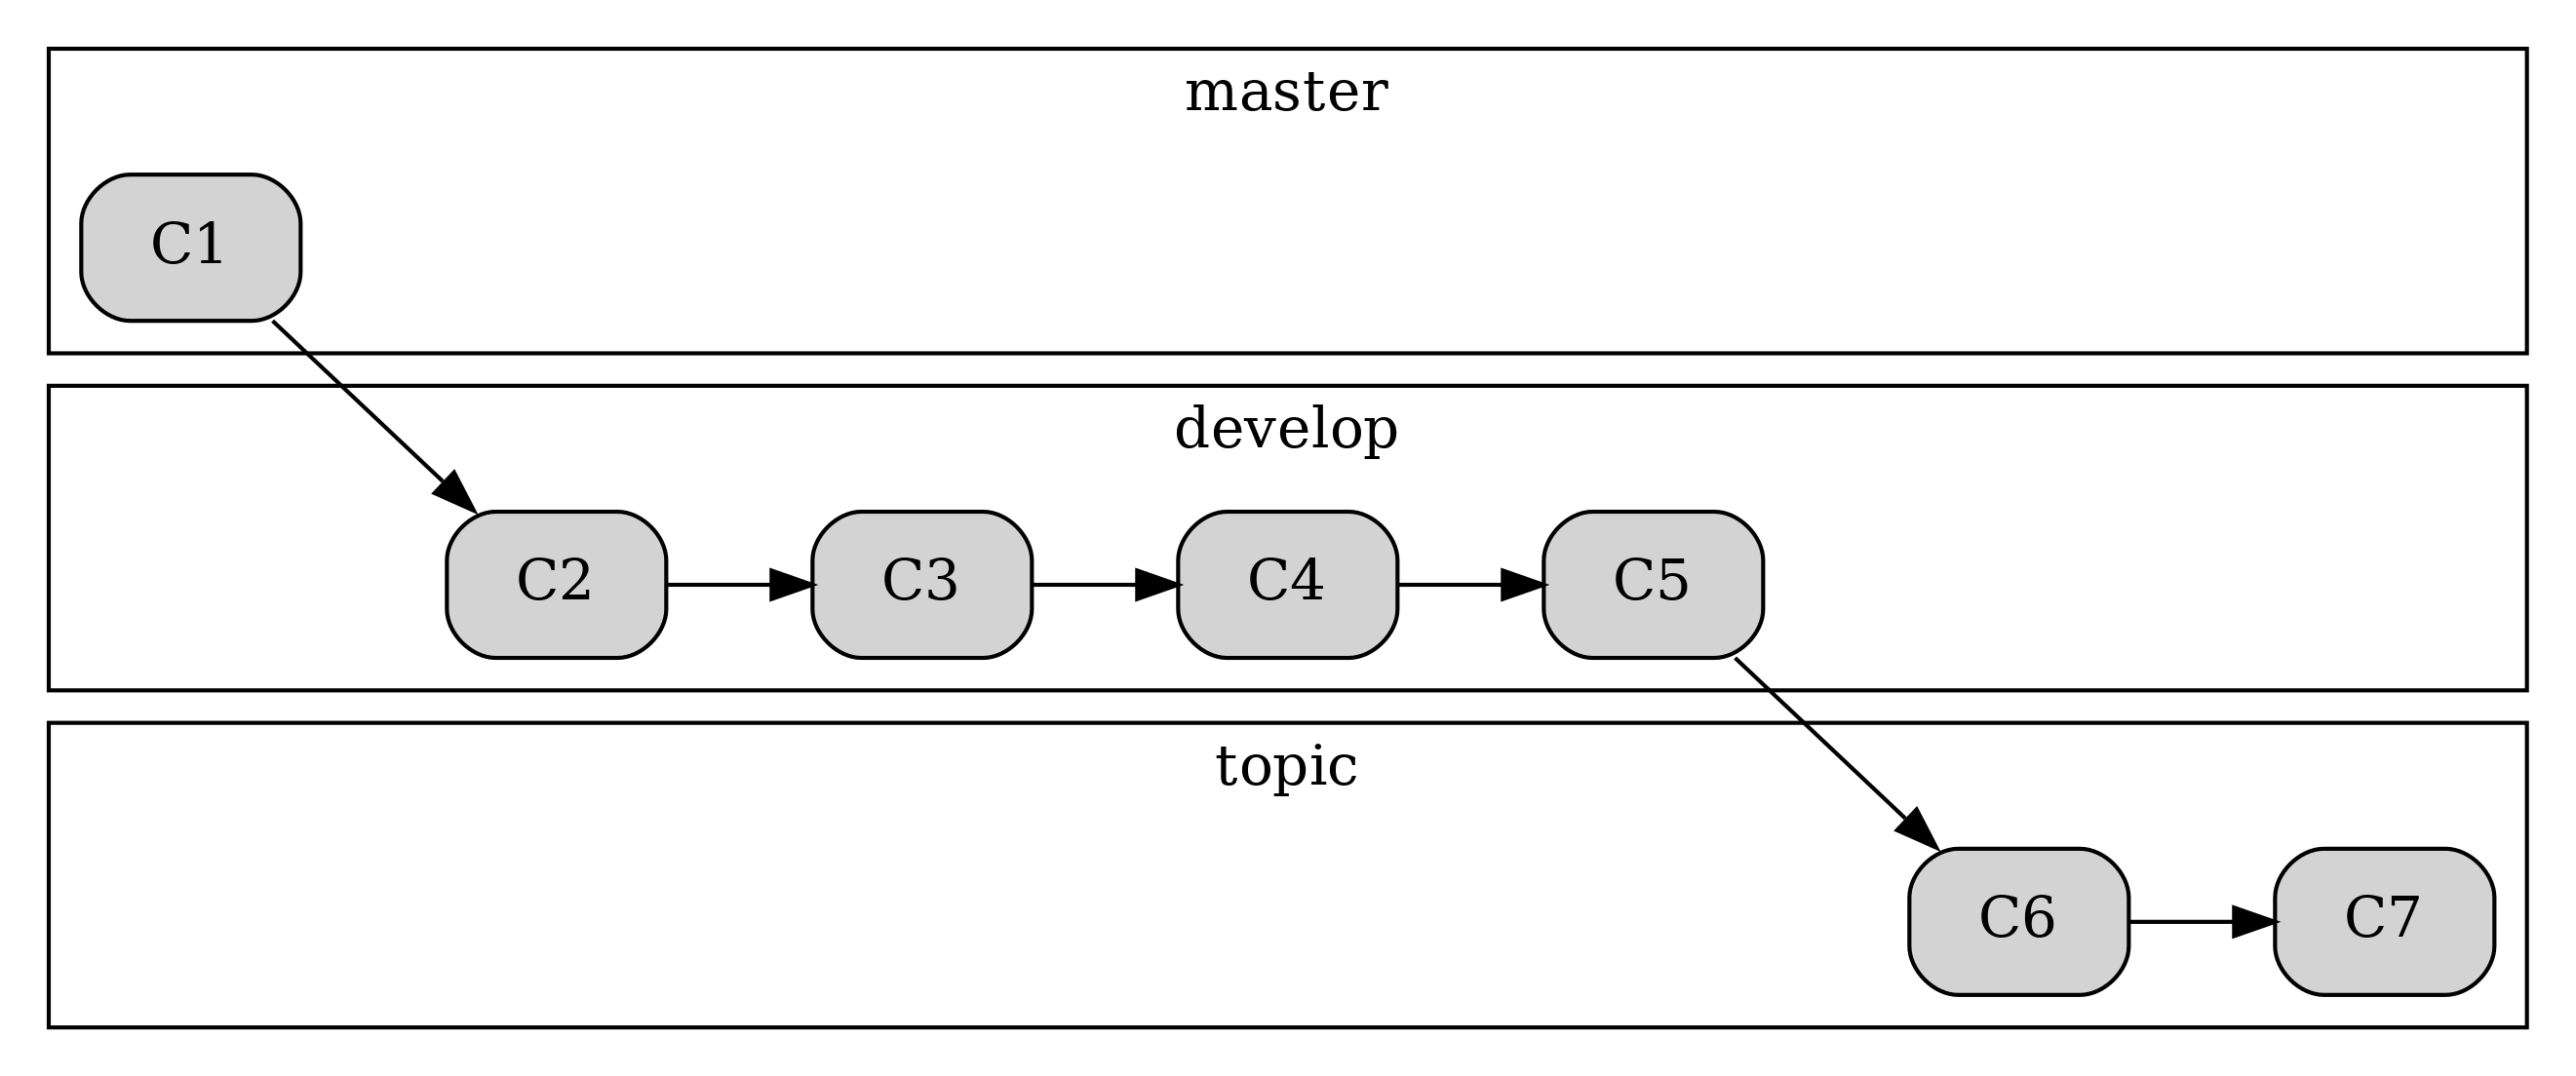
\includegraphics[width=12cm, keepaspectratio]{graphs/git_22.png}
		\end{center}}
	\end{frame}
	
	\begin{frame}{Több ág összeolvasztása}
		\begin{columns}
			\begin{column}{0.4\textwidth}
				\begin{center}
					\begin{block}{Összeolvasztás}
						Az összeolvasztás (\textbf{merge}) a Git verziókezelő rendszerben egy olyan művelet, amelynek során egyik ágból a másikba importálódnak a változtatások. Az összeolvasztás folyamatában a Git megpróbálja összehangolni a különböző ágakban végzett módosításokat, hogy azokat egyetlen, integrált állapotban rögzítse.
					\end{block}
				\end{center}
			\end{column}
			\begin{column}{0.6\textwidth}
				Az 53-as probléma munkája befejeződött és készen áll arra, hogy a főprogrammal együtt legyen kezelve. Ahhoz, hogy ezt meg lehessen tenni, össze kell olvasztani az \textbf{iss53} ágat a \textbf{master} ággal.
				\begin{center}
					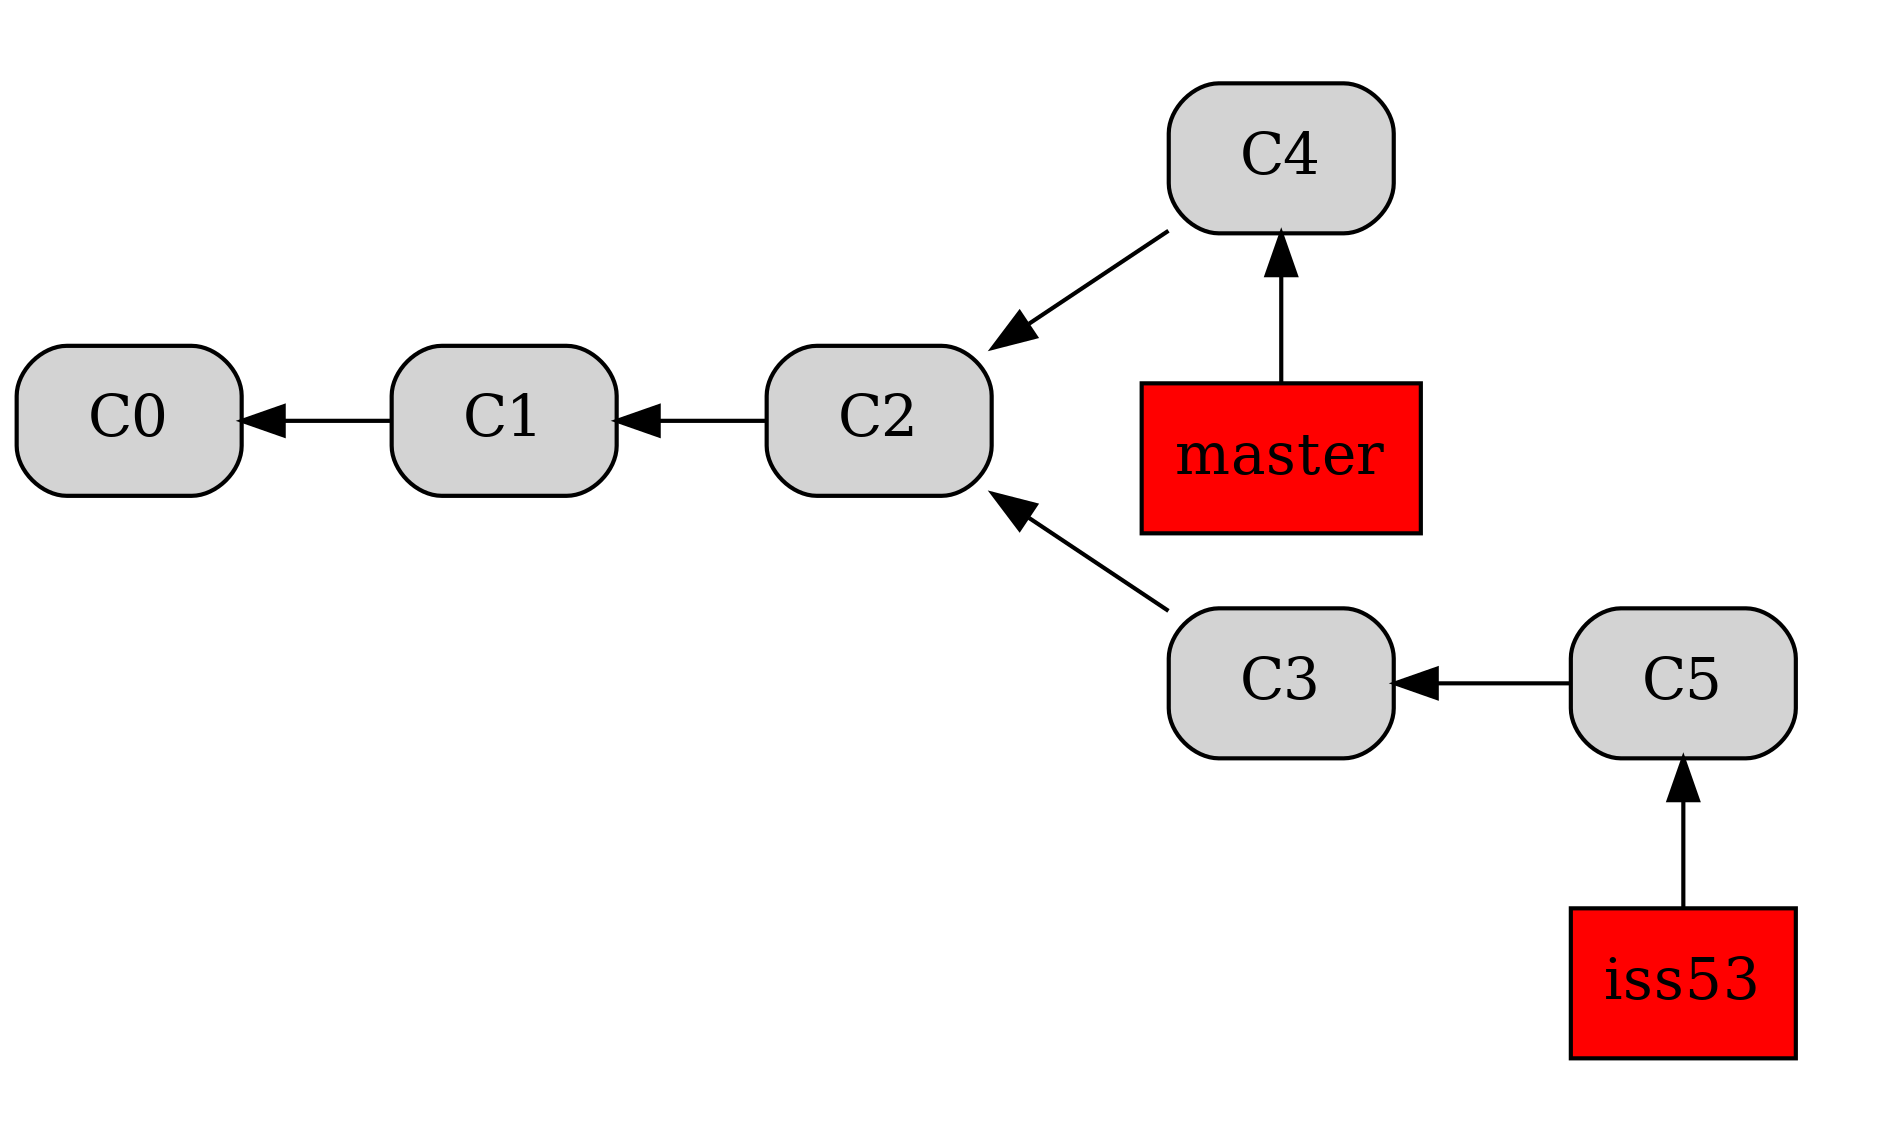
\includegraphics[height=6cm, width=8cm, keepaspectratio]{graphs/git_15.png}
				\end{center}
			\end{column}
		\end{columns}
	\end{frame}
	
	\begin{frame}{Megjelölés összeolvasztásra}
		Mivel a master ágon lévő commit nem közvetlen őse az összeolvasztásra kerülő ágnak, a Gitnek el kell végeznie némi munkát. Ebben az esetben a Git egyszerű háromutas összeolvasztást végez, a két ág pillanatképeire mutató referenciák és a két ág közös őse alapján.
		\begin{center}
			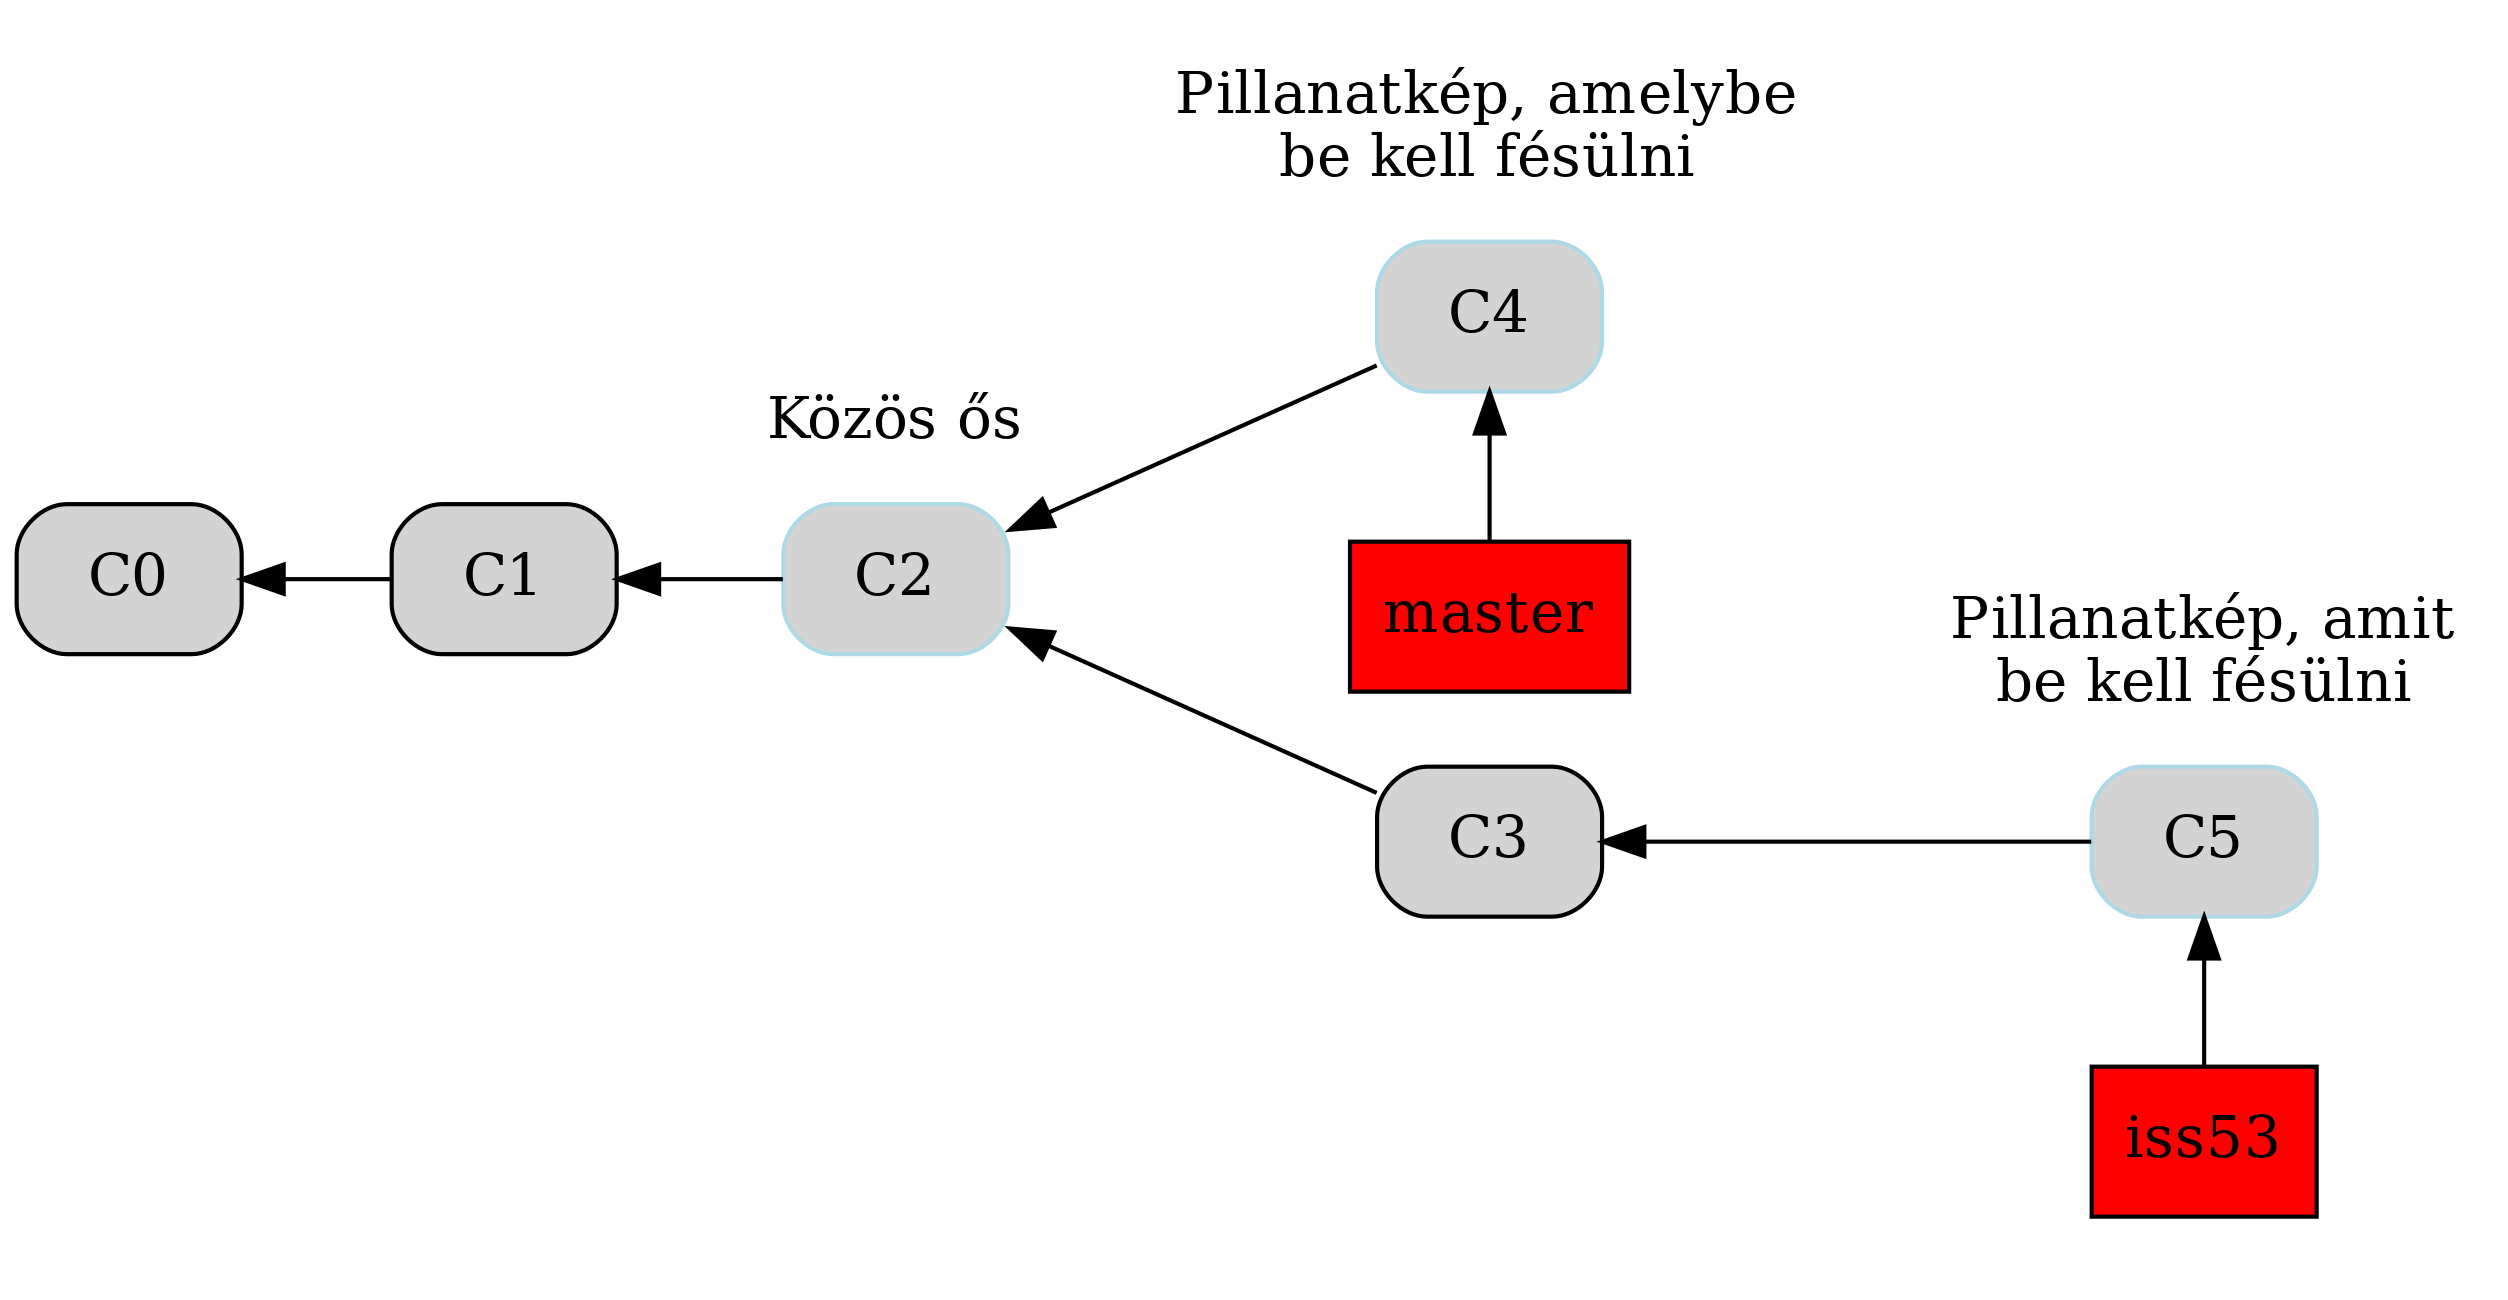
\includegraphics[height=5cm, width=13cm, keepaspectratio]{graphs/git_16.png}
		\end{center}
	\end{frame}
	
	\begin{frame}{Összeolvasztás befejezése}
		Ahelyett, hogy egyszerűen előre mozgatná az ág mutatóját, a Git létrehoz egy új pillanatképet, amely az ebből a háromutas összeolvasztásból ered, és automatikusan létrehoz egy új commitot, amely erre mutat. Ezt nevezzük \textbf{összeolvasztási commitnak}, és különlegessége, hogy több mint egy szülője van.
		\begin{center}
			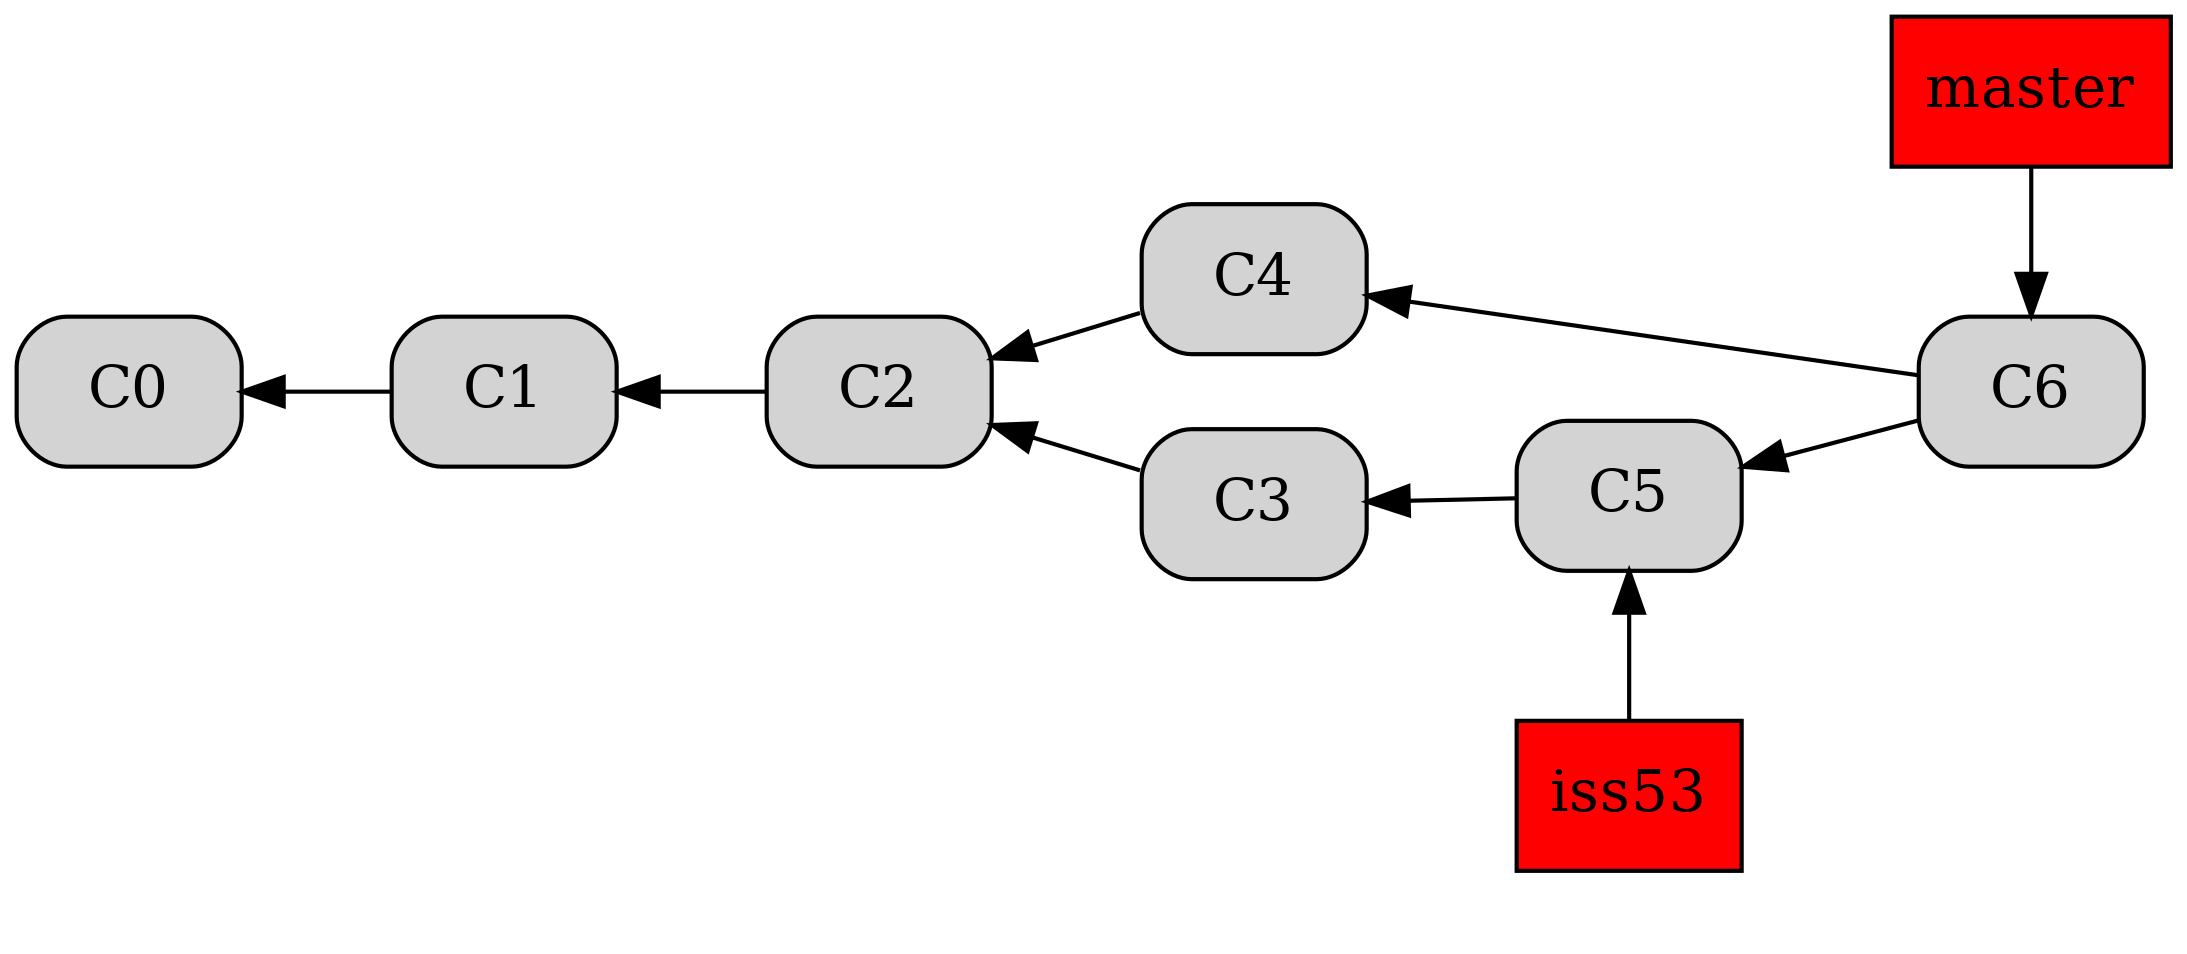
\includegraphics[height=6cm, width=12cm, keepaspectratio]{graphs/git_17.png}
		\end{center}
	\end{frame}
	
	\begin{frame}{Összeolvasztás típusai}
		\begin{columns}
			\begin{column}{0.6\textwidth}
				\begin{itemize}
					\only<1->{\item \textbf{Egyesítés (merge)}: Minden commitot átvesz az összeolvasztandó ágból, és hozzáadja az alapág előzményeihez a létrehozásuk időbélyege alapján.}
					\only<2->{\item \textbf{Összeolvasztás (squash)}: Minden commitot átvesz az ágból és egyetlen commitra olvasztja őket össze. Ez a commit hozzáadódik a történethez, de az ág commitjai közül egyik sem marad meg.}
					\only<3->{\item \textbf{Újra alapozás (rebase)}: Az ág létrehozásának helyét veszi figyelembe, és azt a pontot helyezi át az alapág utolsó commitjára, majd újra alkalmazza a commitokat az ezekre a változásokra.}
				\end{itemize}
			\end{column}
			\begin{column}{0.5\textwidth}
				\begin{center}
					\only<1>{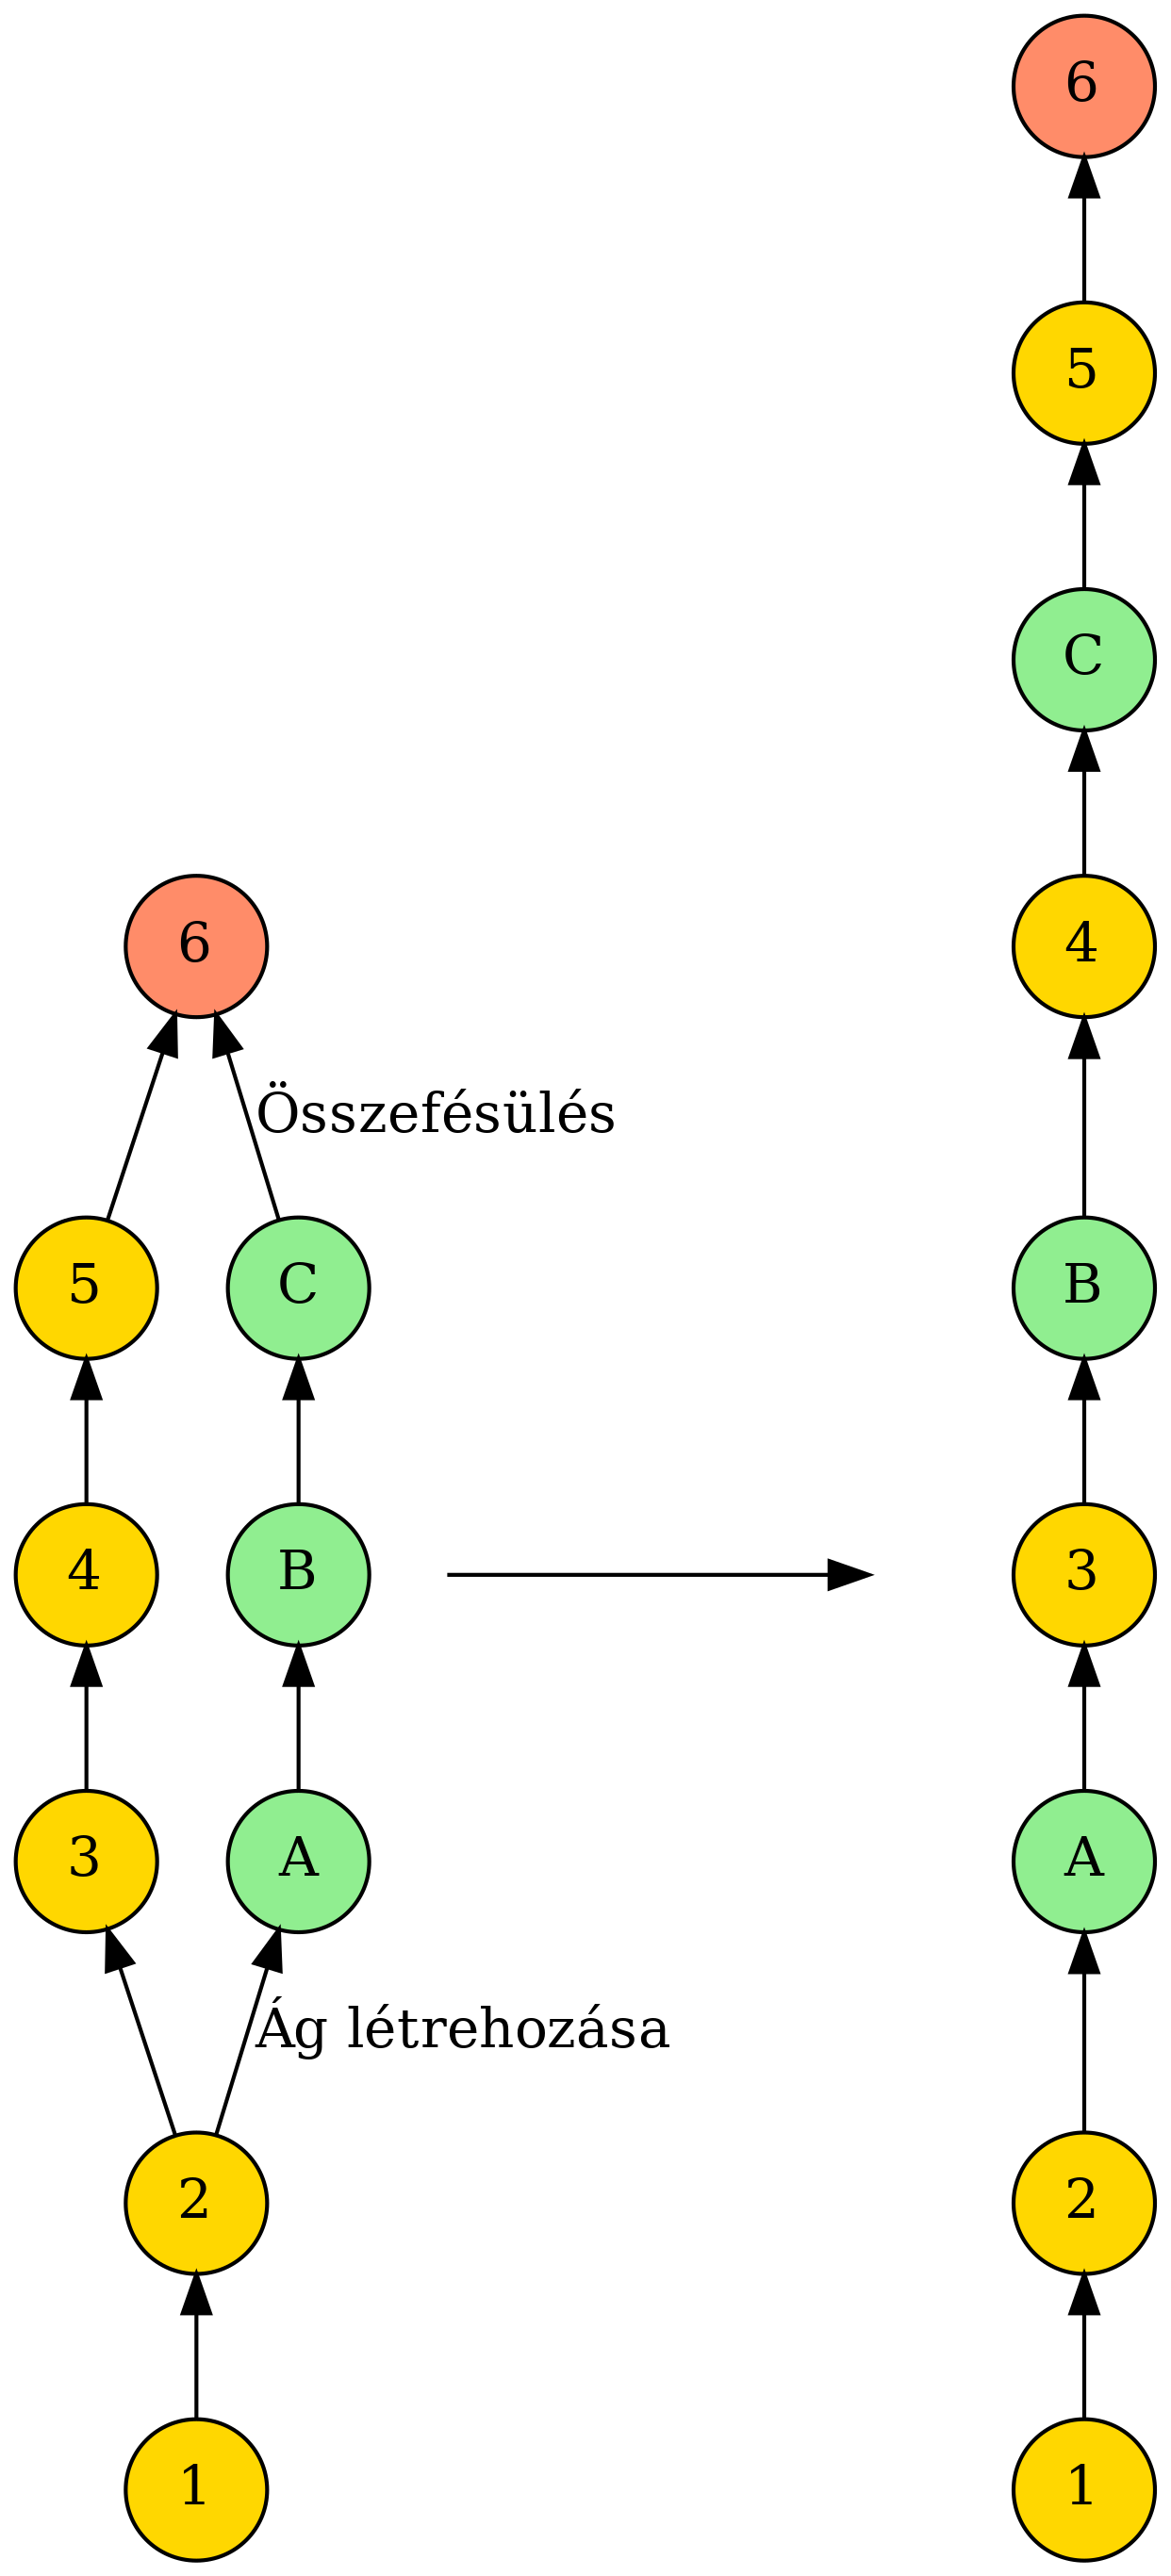
\includegraphics[width=7cm, height=7cm, keepaspectratio]{graphs/git_18.png}}
					\only<2>{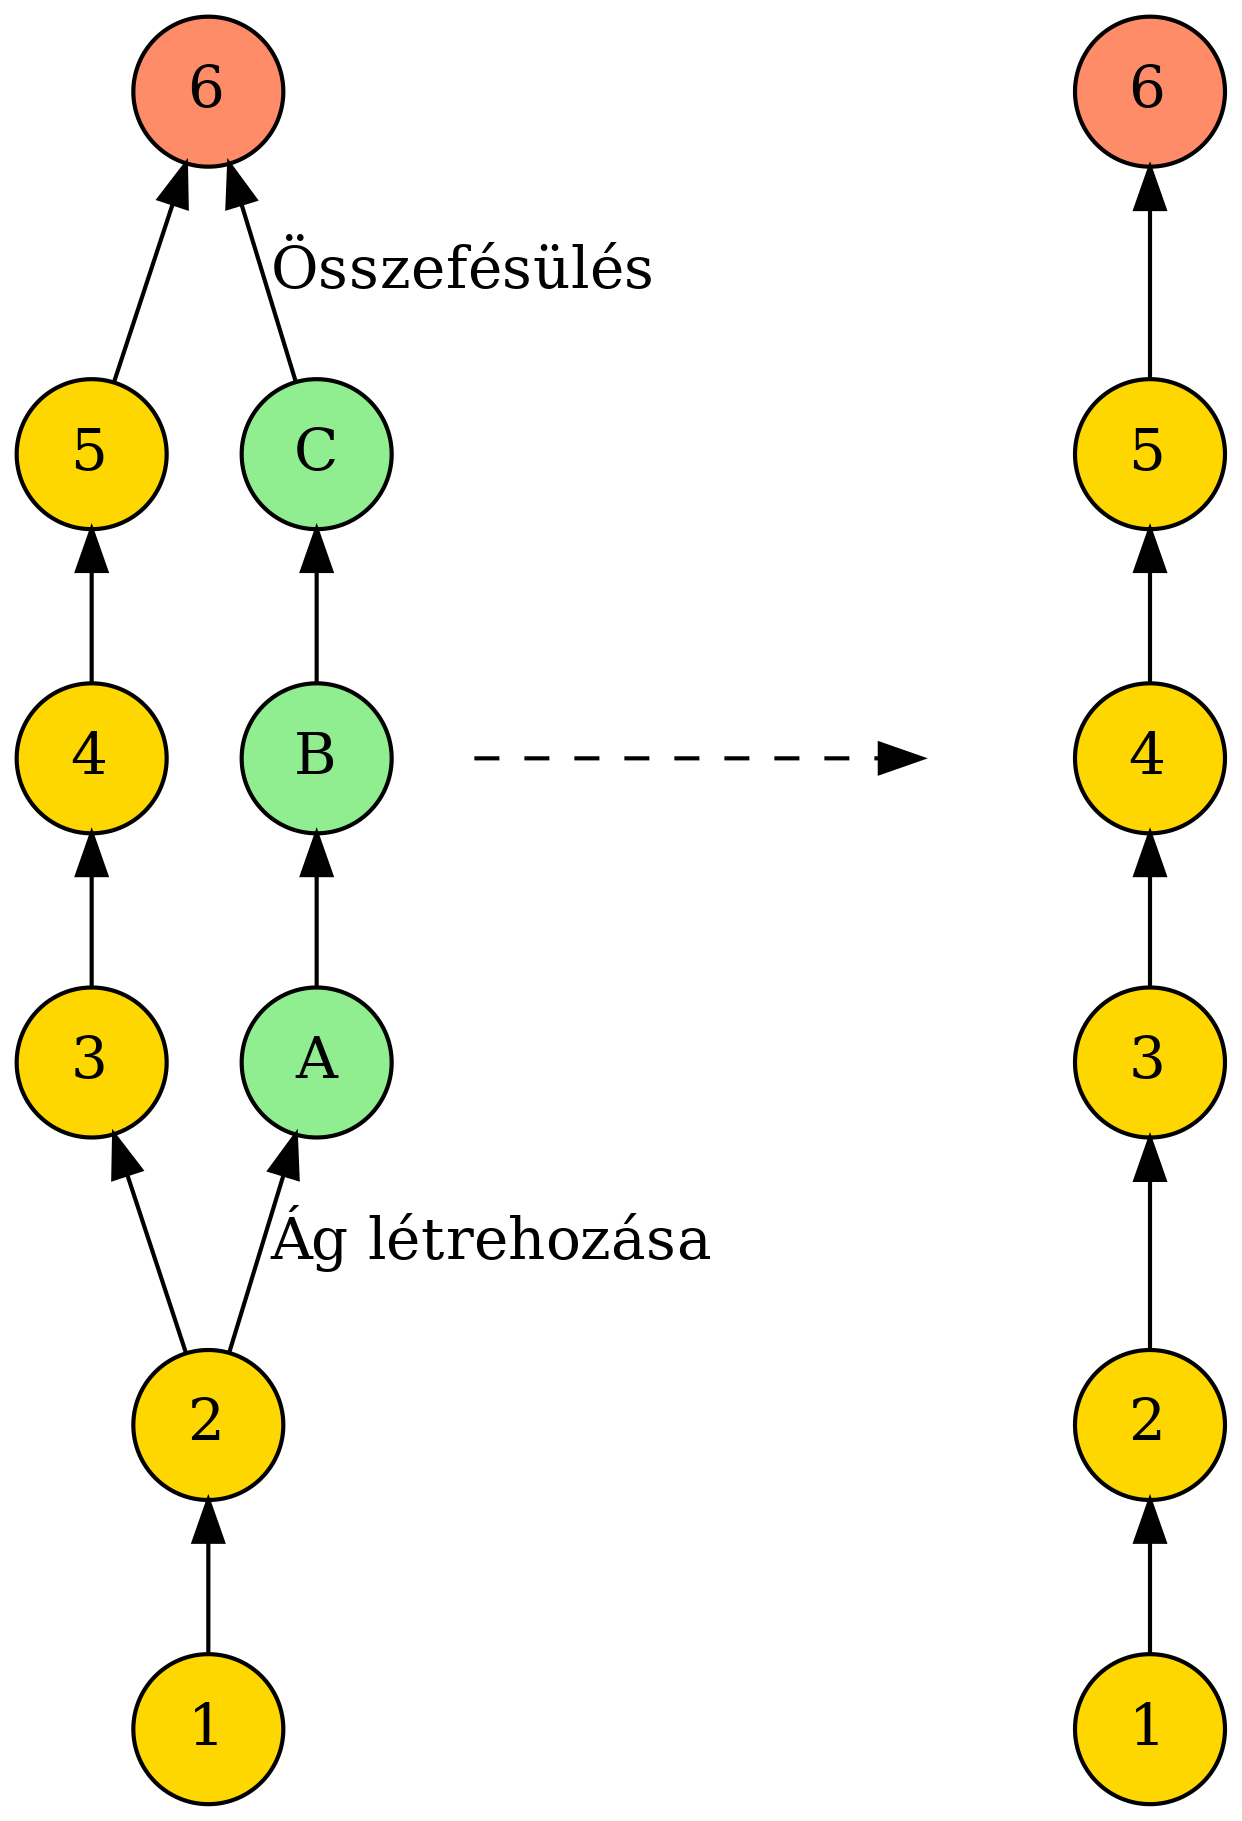
\includegraphics[width=7cm, height=7cm, keepaspectratio]{graphs/git_19.png}}
					\only<3>{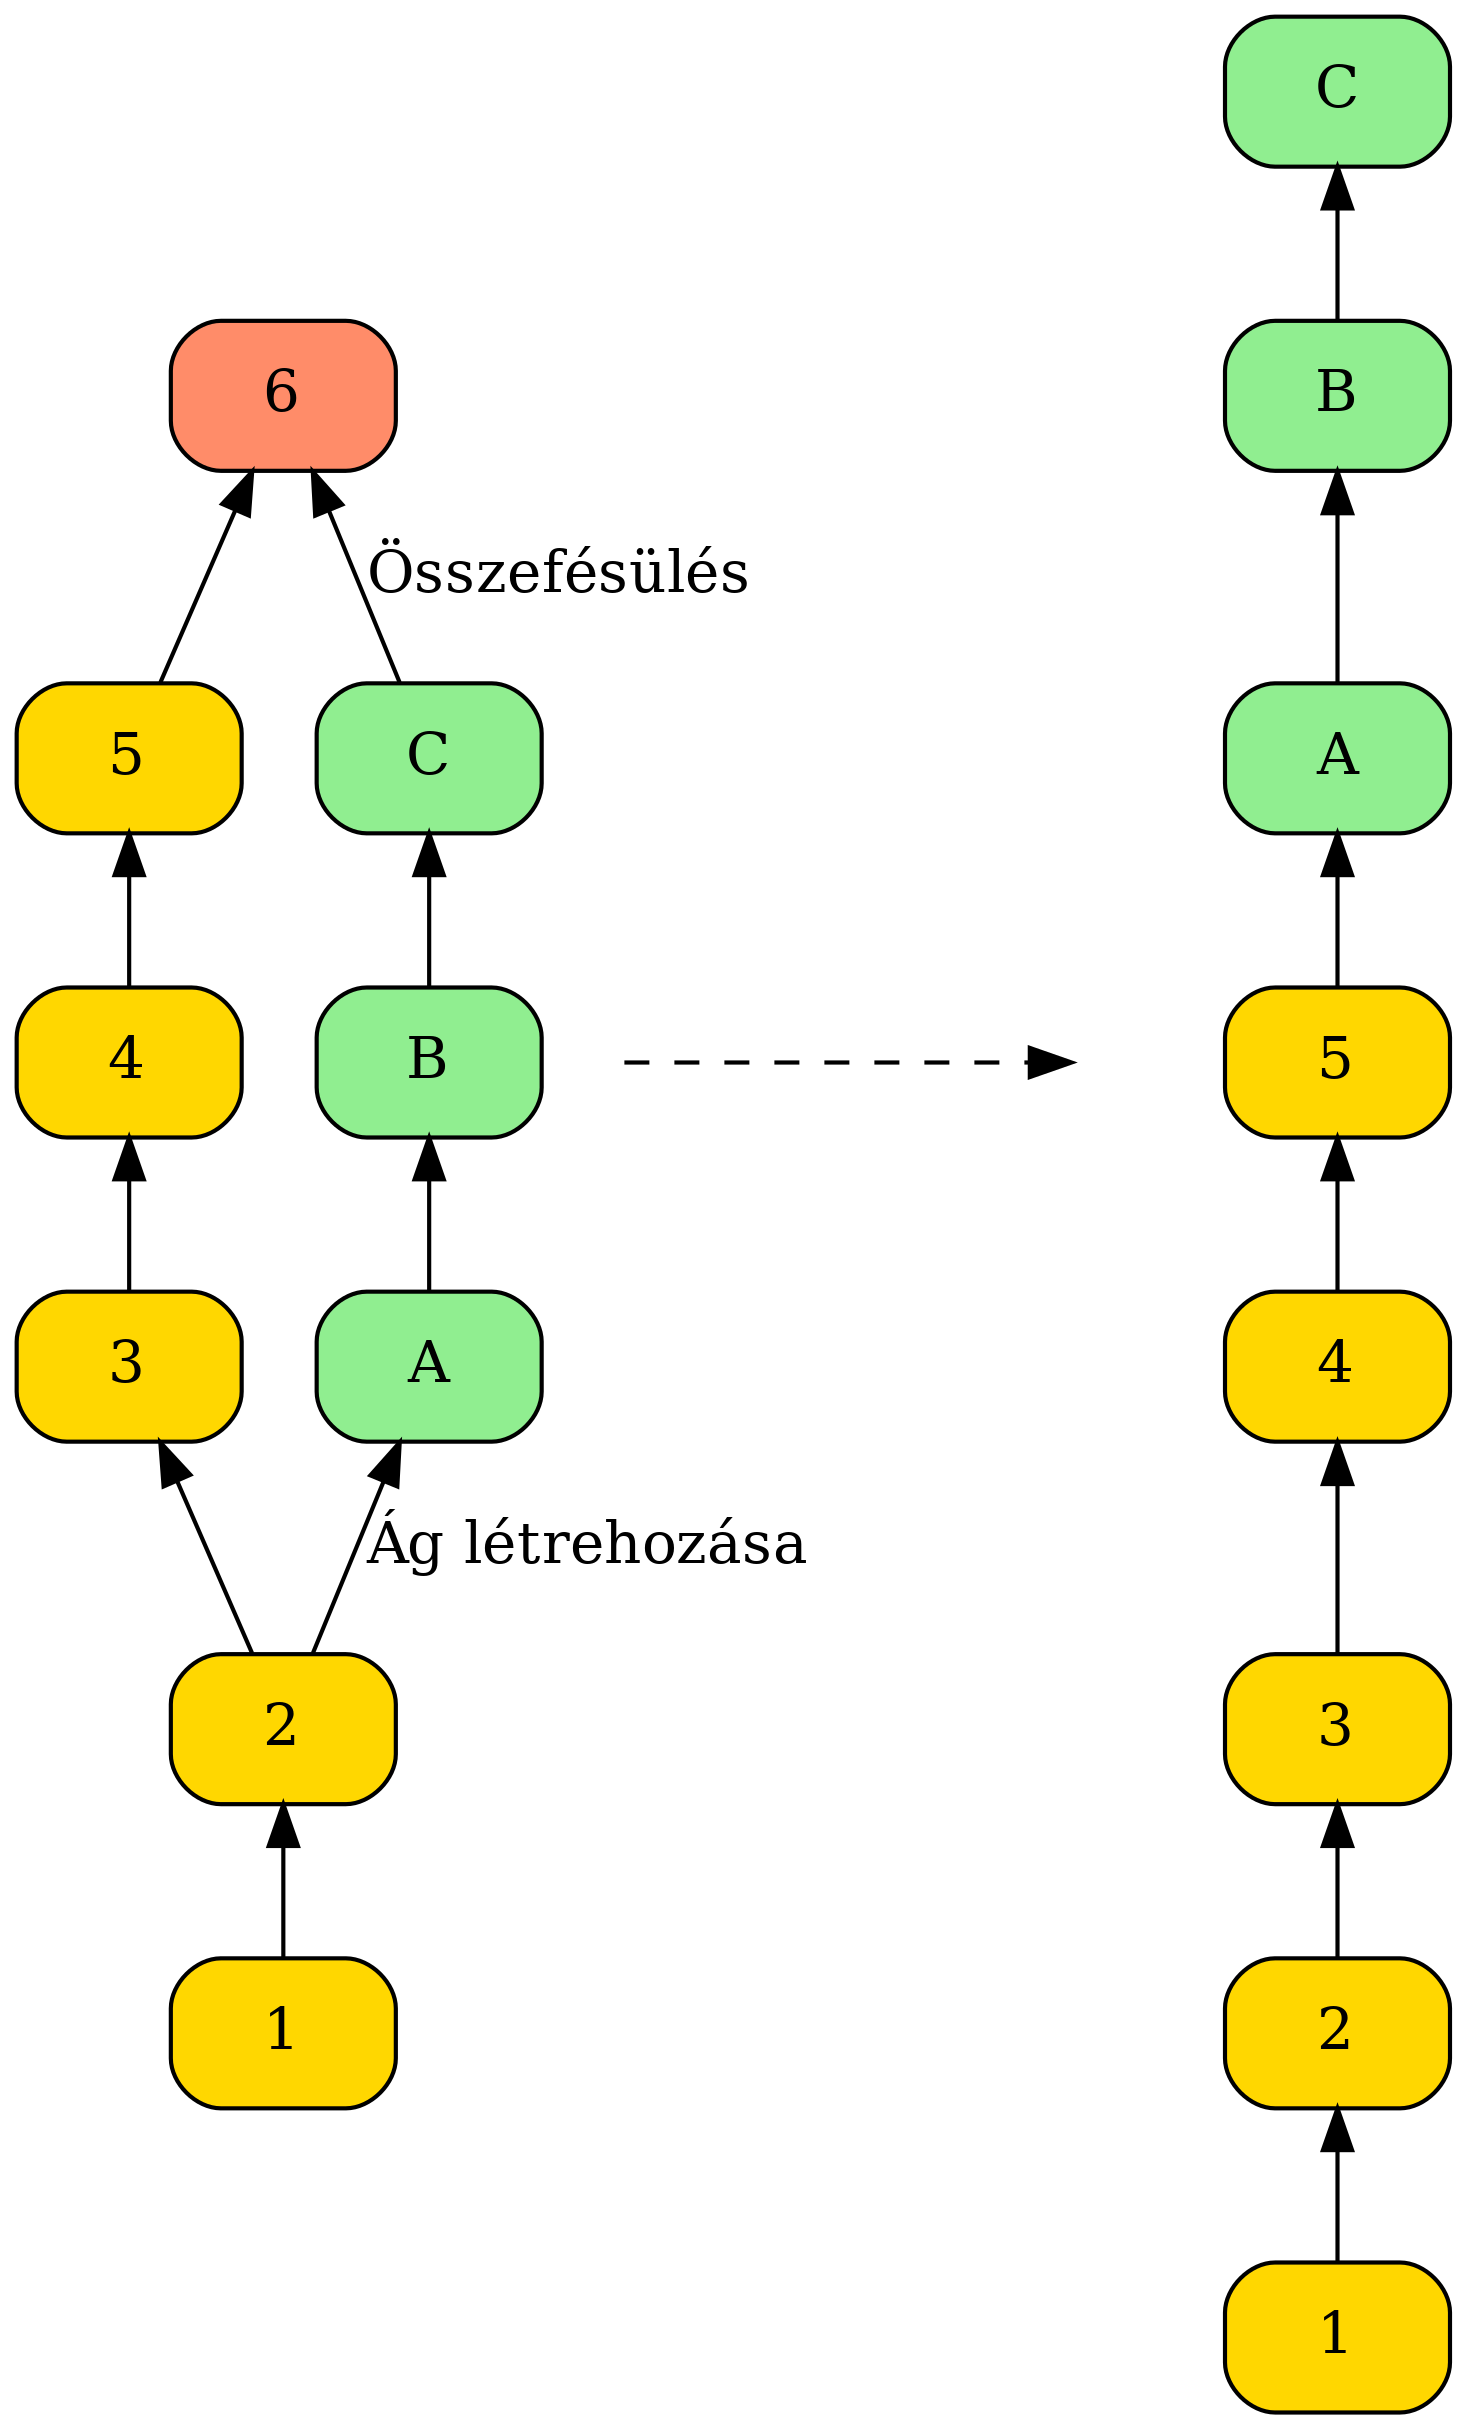
\includegraphics[width=7cm, height=7cm, keepaspectratio]{graphs/git_20.png}}
				\end{center}
			\end{column}
		\end{columns}
	\end{frame}
	
	\section{Összeolvasztási konfliktusok}
	
	\begin{frame}
		\tableofcontents[currentsection]
	\end{frame}
	
	\begin{frame}{Konfliktusok előfordulása}
		\begin{columns}
			\begin{column}{.5\textwidth}
				\begin{footnotesize}
					\begin{block}{}
						\texttt{
							\$ git merge iss53\\
							Auto-merging index.html\\
							CONFLICT (content): Merge conflict in index.html\\
							Automatic merge failed; fix conflicts and then commit the result.\\}
					\end{block}
				\end{footnotesize}
			\end{column}
			\begin{column}{.5\textwidth}
				Időnként az összefésülési folyamat nem megy zökkenőmentesen. Ha ugyanazon fájl ugyanazon részét különböző
				módon módosították a két egyesítendő ágon, a Git nem lesz képes tisztán egyesíteni őket.\\
				\vspace{0.2cm}
				A Git ebben az esetben nem hoz létre összefésülési commitot, hanem leállítja a folyamatot addig, amíg a konfliktust
				manuálisan fel nem oldja a fejlesztő
			\end{column}
		\end{columns}
	\end{frame}
	
	\begin{frame}{Konfliktusok előfordulása}
		\begin{columns}
			\begin{column}{.5\textwidth}
				\begin{footnotesize}
					\begin{block}{}
						\texttt{
							\$ git status\\
							On branch master\\
							You have unmerged paths.\\
							(fix conflicts and run "git commit")\\
							Unmerged paths:\\
							(use "git add <file>..." to mark resolution)\\
							both modified: index.html\\
							no changes added to commit (use "git add" and/or "git commit -a"\\}
					\end{block}
				\end{footnotesize}
			\end{column}
			\begin{column}{.5\textwidth}
				A \texttt{git status} parancs füttatásával lehet látni, melyek azok a fájlok, amelyekben összefésületlen konfliktusok
				találhatóak.\\
				\vspace{0.2cm}
				Minden olyan fájl, amelyikben konfliktus található, összefésületlen státuszba kerül.
			\end{column}
		\end{columns}
	\end{frame}
	
	\begin{frame}[fragile]\frametitle{Konfliktusok jelölése fájlokban}
		\begin{columns}
			\begin{column}{.5\textwidth}
				\begin{footnotesize}
					\begin{block}{}
						\begin{verbatim}
<<<<<<< HEAD:index.html
<div id="footer">contact :
email.support@github.com</div>
=======
<div id="footer">
please contact us at support@github.com
</div>
>>>>>>> iss53:index.html
						\end{verbatim}
					\end{block}
				\end{footnotesize}
			\end{column}
			\begin{column}{.5\textwidth}
				A konfliktusos fájlok megfelelő részeiben ehhez hasonló szekciók lesznek találhatóak, amik jelzik a különbséget a két ág, ebben az esetben a \texttt{master} és a \texttt{iss53} között.\\
				\vspace{0.2cm}
				A programozónak olyan formára kell hoznia a fájlokat, hogy a konfliktus feloldódjon a megfelelő részek kitörtésével.
			\end{column}
		\end{columns}
	\end{frame}
	
	\section{Távoli fejlesztési ágak}
	
	\begin{frame}
		\tableofcontents[currentsection]
	\end{frame}
	
	\begin{frame}{Távoli tárhely lemásolása (\texttt{clone})}
		Ha van egy Git szerver a hálózaton a \texttt{git.company.com} címen, innen a Git képes automatikusan letölteni a az összes adatot. A távoli tárhelyet a Git \texttt{origin} néven nevezi el, és létrehoz egy mutatót a \texttt{master} ágra. Lokálisan \texttt{origin/master} néven inicializál mutatót egy helyi \texttt{master} ágra.
		\begin{center}
			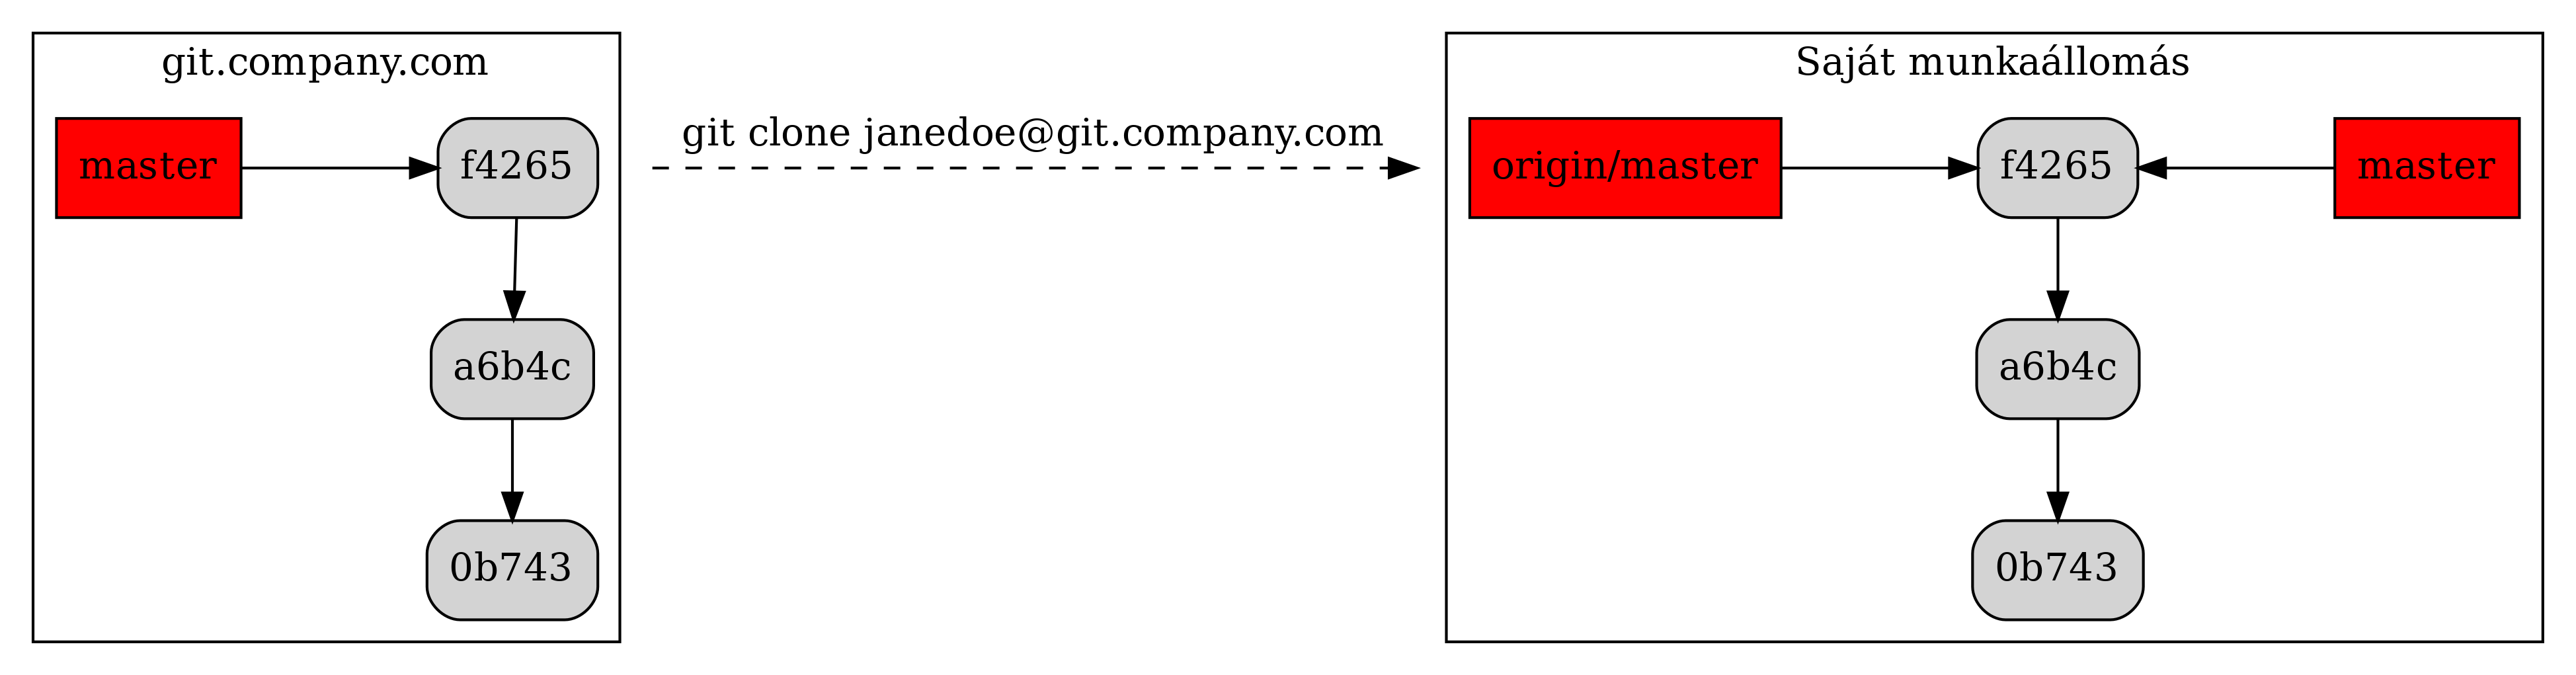
\includegraphics[width=14cm]{graphs/git_23.png}
		\end{center}
	\end{frame}
	
	\begin{frame}{Fejlesztés a távoli ágon (\texttt{commit})}
		\begin{columns}
			\begin{column}{.5\textwidth}
				Ha a lokális \texttt{master} ágon történő munka közben egy másik fejlesztő feltölt változtatást a \texttt{git.company.com} szerverre és frissítani annak \texttt{master} ágát, a két fejlesztési történet divergál.\par\smallskip
				Amíg nem töltődnek le a frissítések a távoli szerverről, a helyi \texttt{master} mutató változatlan marad.
			\end{column}
			\begin{column}{.5\textwidth}
				\begin{center}
					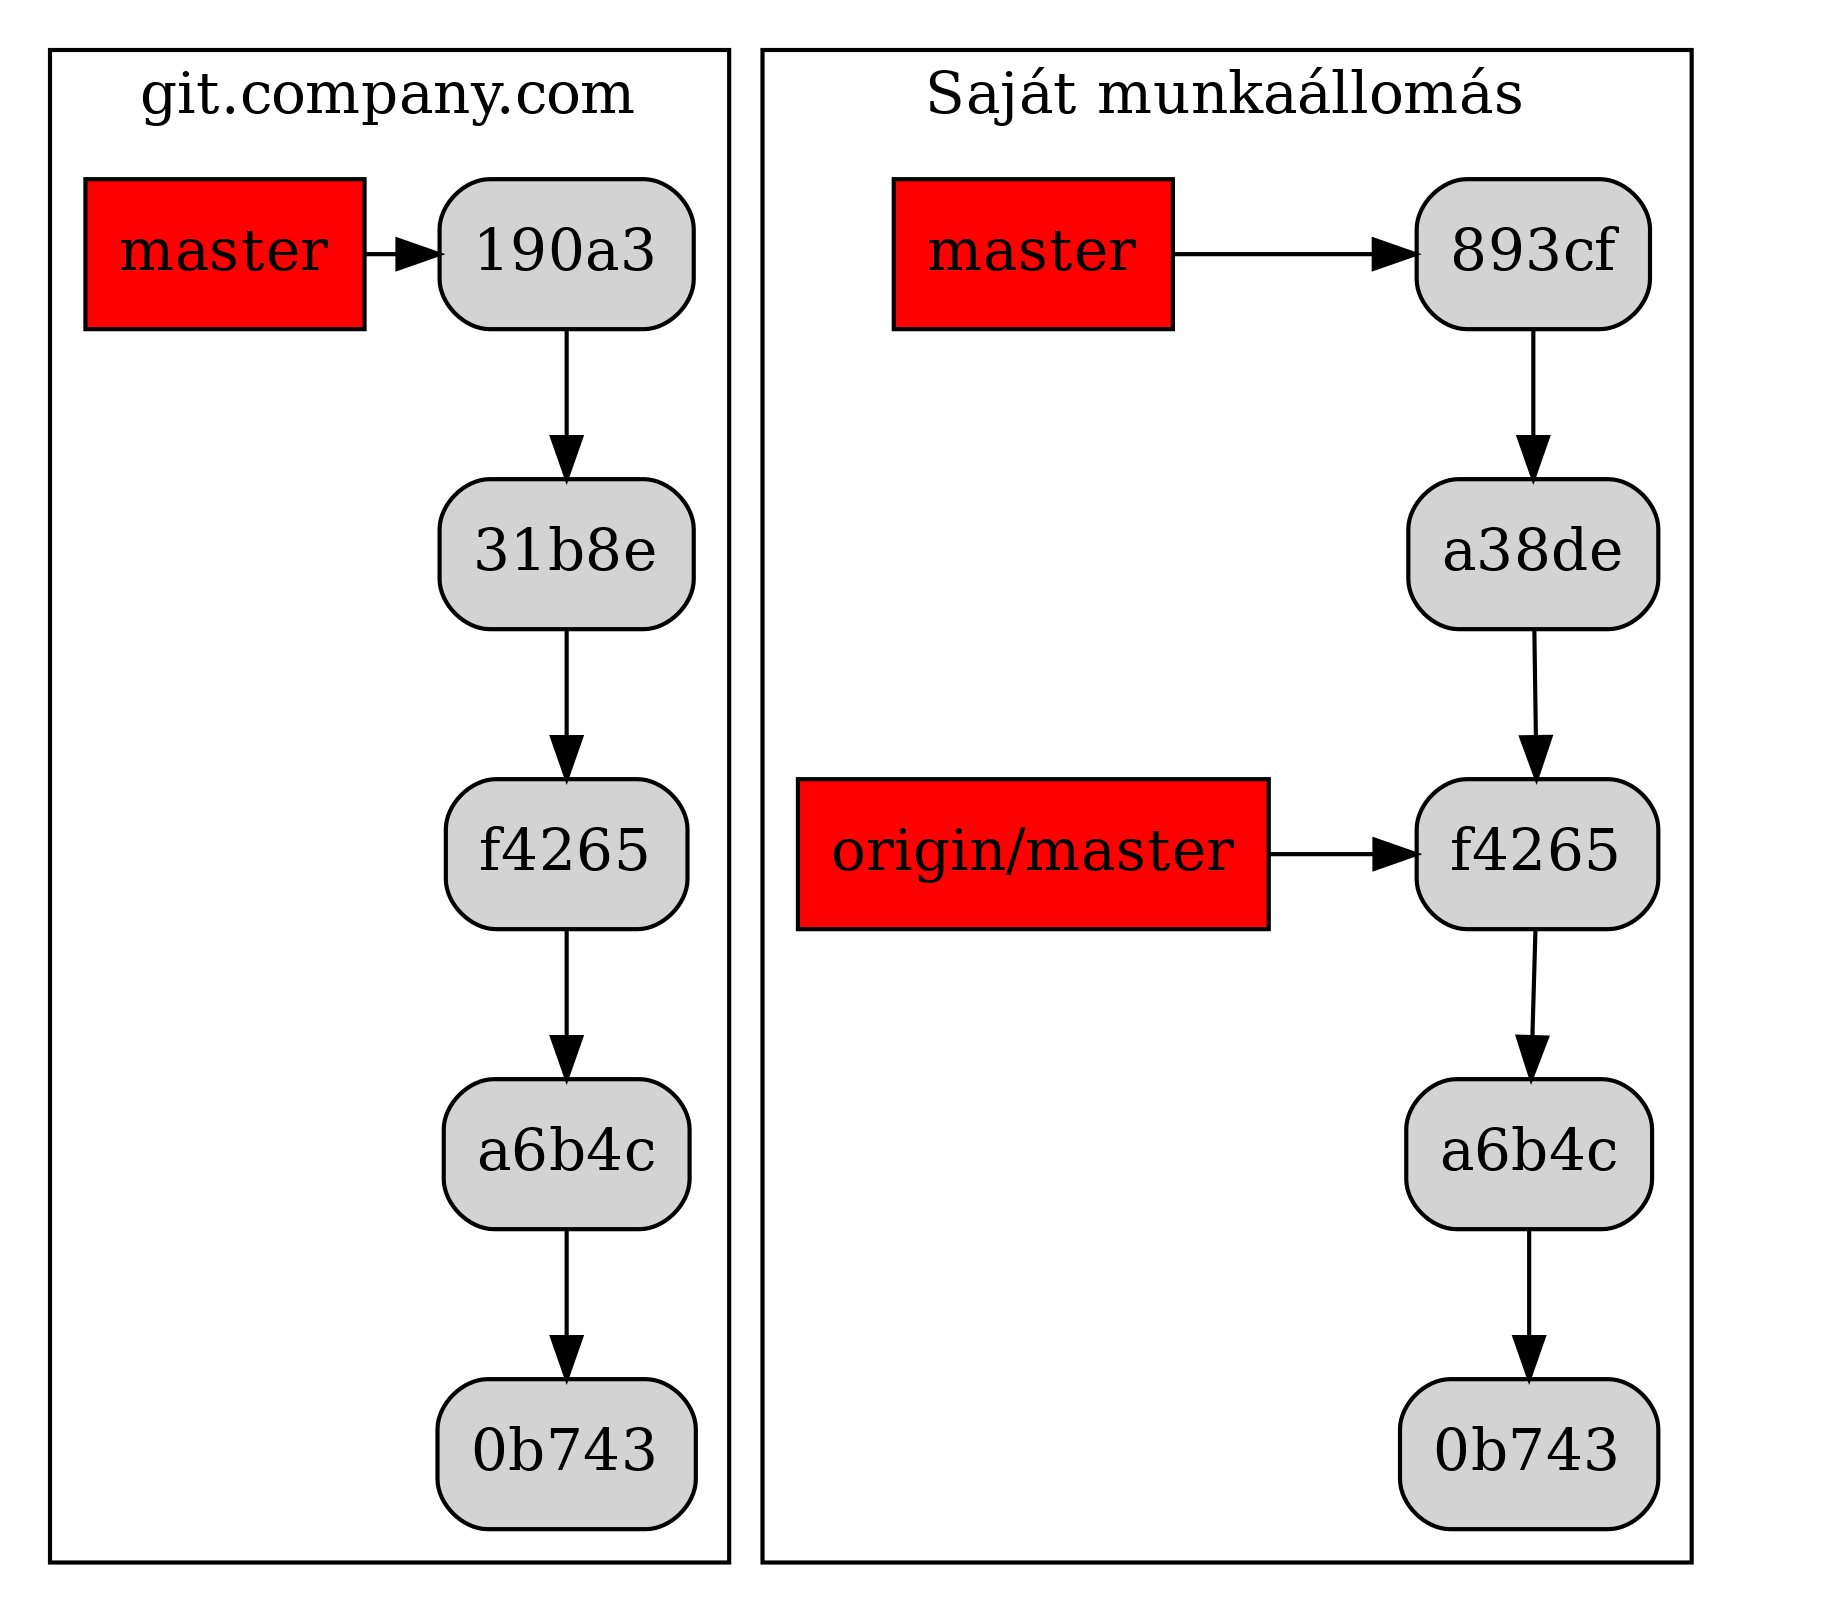
\includegraphics[width=7cm, height=7cm, keepaspectratio]{graphs/git_24.png}
				\end{center}
			\end{column}
		\end{columns}
	\end{frame}
	
	\begin{frame}{Két ág szinkronizálása (\texttt{fetch})}
		Ágak szinkronizálását a \texttt{git fetch} parancs teszi lehetővé. Ez az utasítás megkeresi, hogy melyik szerver az \texttt{origin} (jelen esetben a \texttt{git.company.com}), letölti azokat az adatokat, amelyek még nincsenek jelen a lokális munkaállomáson, frissíti a helyi adatbázist és az \texttt{origin/master} mutatót naprakész pozícióba helyezi.
		\begin{center}
			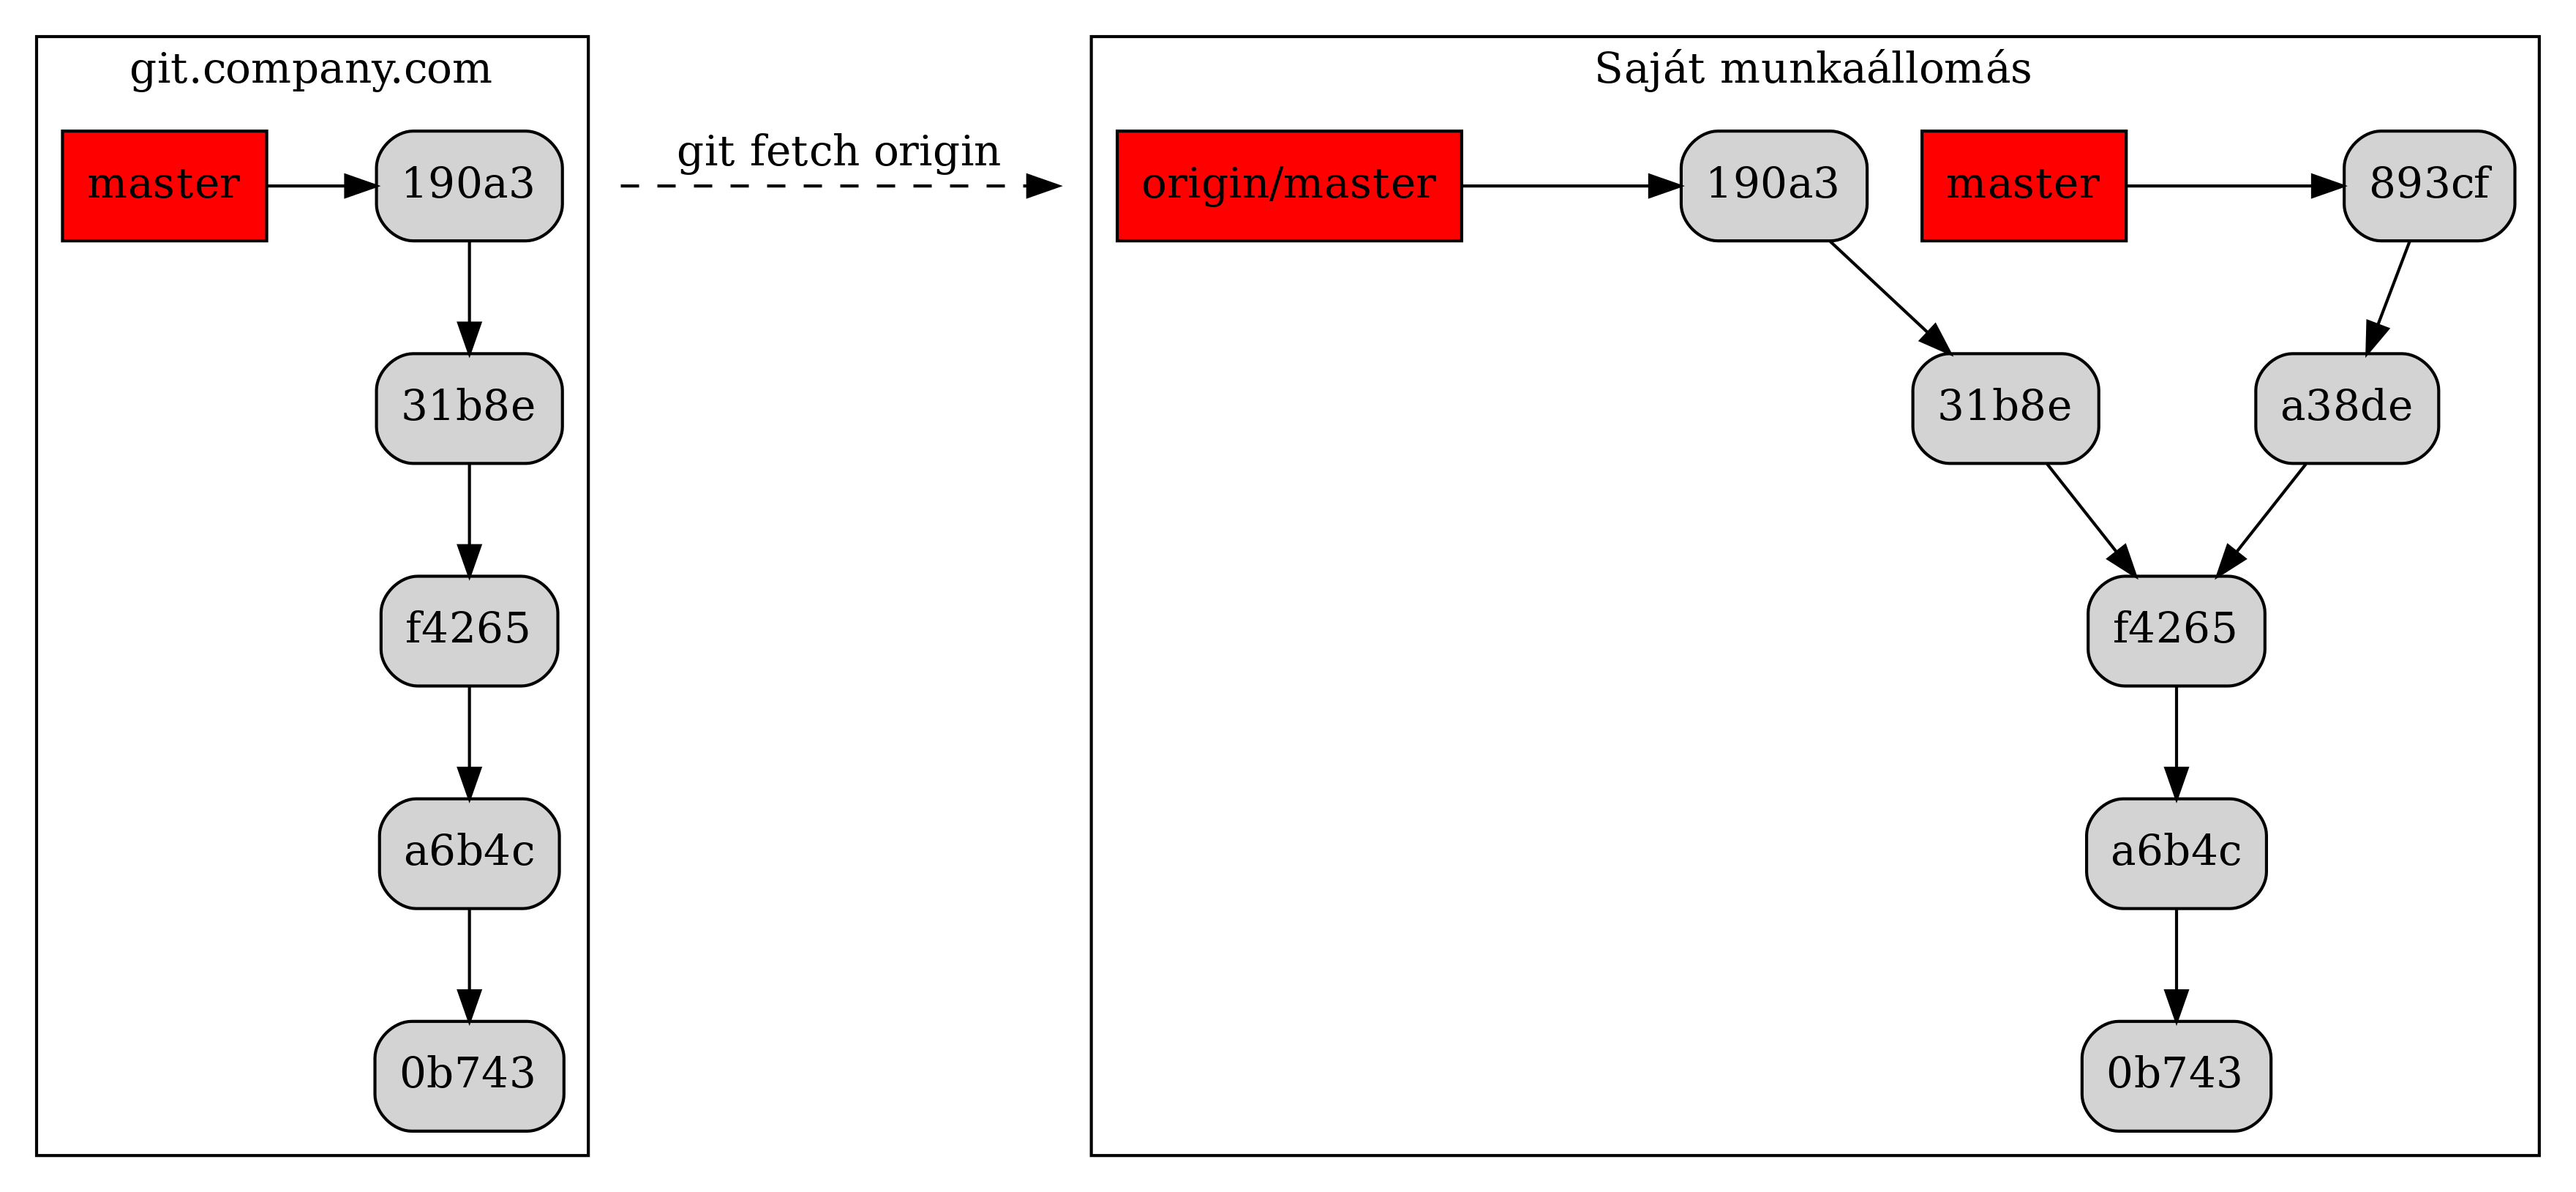
\includegraphics[width=10.5cm, keepaspectratio]{graphs/git_25.png}
		\end{center}
	\end{frame}
	
	\begin{frame}{Harmadik ág szinkornizálása (\texttt{fetch})}
		Ha a programozó a \texttt{git fetch teamone} parancsot futtatja, hogy letöltsön minden, a \texttt{teamone} ágon található adatot, a Git nem kér le új adatot, mert már rendelkezik az \texttt{origin} szerveren található adatok egy részhalmazával. Egy új mutató inicializálódik, \texttt{teamone/master} néven, ami arra a commitra mutat, amelyet a \texttt{teamone} szerver \texttt{master} néven tart nyilván.
		\begin{center}
			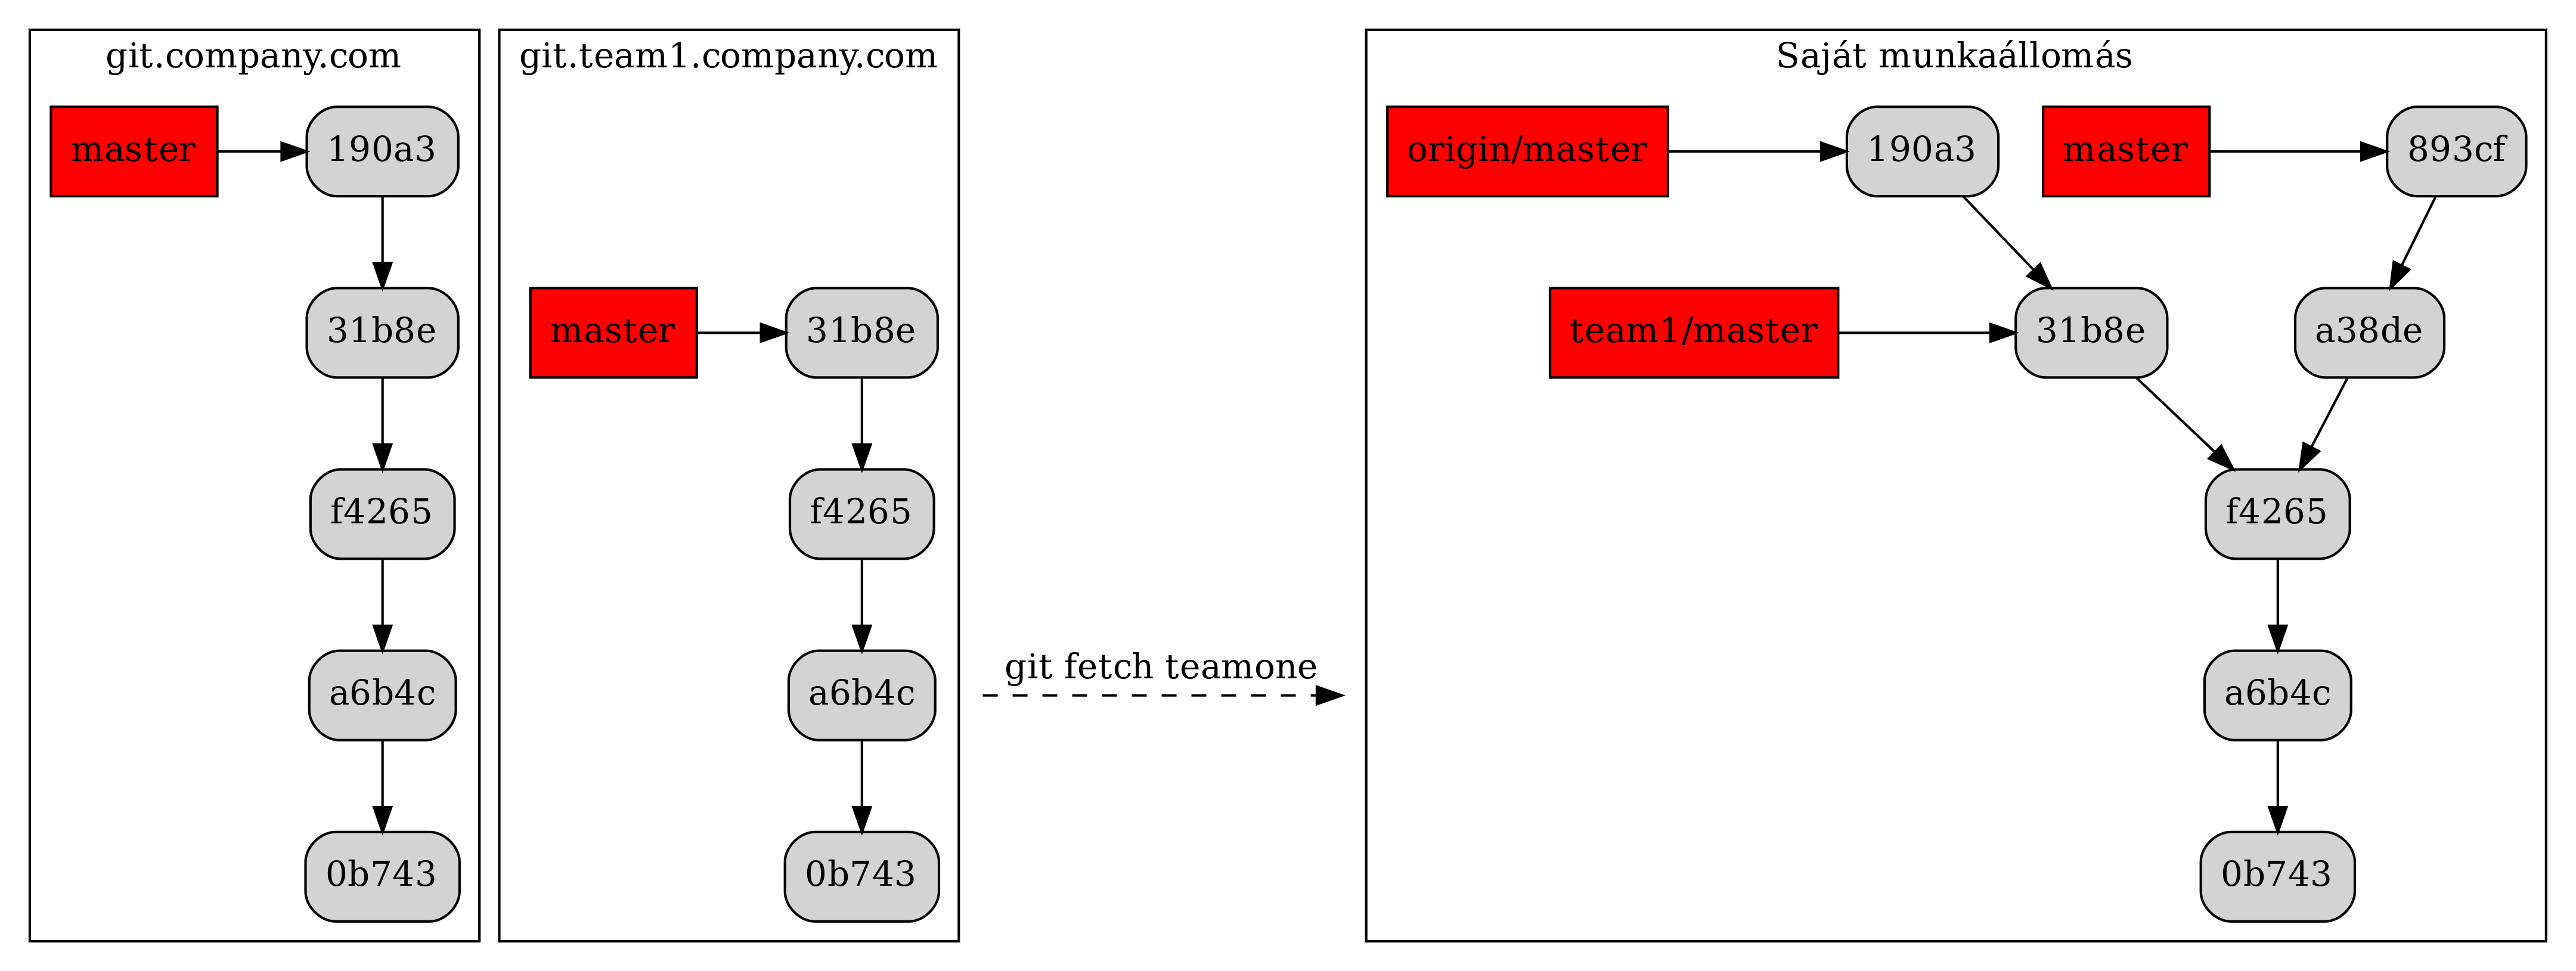
\includegraphics[width=12cm, keepaspectratio]{graphs/git_26.png}
		\end{center}
	\end{frame}
	
	\begin{frame}{Változtatások véglegesítése}
		\begin{columns}
			\begin{column}{.5\textwidth}
				\begin{block}{\texttt{push}}
					A \texttt{git push} parancs a lokális fájlrendszeren végrehajtott változtatásokat feltölti a távoli tárhelyre. Ezáltal a commitok és ágak szinkronizálódnak a repozitóriummal.
				\end{block}
			\end{column}
			\begin{column}{.5\textwidth}
				\begin{block}{\texttt{pull}}
					A \texttt{git pull} parancs a távoli repozitóriumban lévő változtatások letöltésére és a helyi repozitóriummal való egyesítésére szolgál.\par \smallskip
					Ez a parancs valójában két műveletet hajt végre: először a \texttt{git fetch} parancsot, amely letölti a változtatásokat, majd a \texttt{git merge} parancsot, amely egyesíti azokat a helyi ággal.
				\end{block}
			\end{column}
		\end{columns}
	\end{frame}
\end{document}